% Main thesis document
\documentclass[a4paper, 11pt]{report}

\usepackage{include}
\usepackage{definitions}
\usepackage[thesistype=master]{chalmersthesis}

\addbibresource{bibliography.bib}

% Define title specific author fields
\title{Symmetries of Mathematical Models in Biology}
\author{Felix Augustsson}
\examiner{Marija Cvijovic}
\supervisor{%
  Johannes Borgqvist\thanks{Mathematical Institute, University of Oxford} \and%
  Fredrik Ohlsson\thanks{Department of Mathematics and Mathematical Statistics, Umeå University} \and%
  Marija Cvijovic%
}
\department{Department of Mathematical Sciences}
\degree{Engineering Mathematics and Computational Science}
\date{2021}
\illustration{images/cover}
\illustrationdescription{
  The jet surfaces of the classical and autonomous Gompertz models, with representative transformations of respective Lie point symmetries, acting on a common solution curve of the two model formulations.
  Generated with Matplotlib in Python, with code availible at the repository described in \cref{app:computer-algebra}.
}
\setabstract{
  In biology, a common type of mathematical model is systems of first order ordinary differential equations (ODE:s).
  In general, large non-linear systems of ODE:s have no analytic solutions.
  Mathematical symmetries can however still be used to analytically study differential equations, without the need to find explicit solutions.
  Symmetries are transformations that map solutions of a differential equation to other solutions, and thus contain a lot of information about the system.
  However, due to the historical development of the theory of symmetries alongside physics, the literature on finding symmetries of the type of large systems of first order ODE:s usually found in biology is sparse.

  In this thesis, four biological models using first order ODE:s are studied using Lie point symmetries: the Hill equation, the Gompertz model, the Lotka-Volterra predator--prey model and the Yildirim--Mackey lactose operon model.
  Symmetries of all models are found using ansätze.
  Additionally, symmetries are found using a repurposed method based on parameter independence.
  It is also shown that, using both methods for finding symmetries, sophisticated computer algorithms are needed for the calculation of symmetries of bigger systems to be viable.

  Additionally, the general structure of symmetries is investigated for different formulations of the Gompertz model.
  It is shown that the two scalar Gompertz model formulations found in literature are symmetrically special cases of the original system formulation, and the consequence for model building in biological systems is discussed.

  It is concluded that due to the generality of the mathematical theory, symmetries show promise of being a useful tool when studying mathematical models in biology.
  However, several mathematical problems have to be solved before symmetries can be used in day--to--day biological modeling.
}

\begin{document}

\maketitle

\pagenumbering{roman}

\tableofcontents

\clearpage
\pagenumbering{arabic}
\setcounter{page}{1}

\addsec{Introduction}

In many scientific fields the concept of symmetry is important.
Symmetries bridge the gap between the qualitative and the quantitative; it is both a statement about what a system is, and how a system can be measured.
In most cases when symmetries are discussed, the symmetries in question are simple, geometric symmetries.
These can be mirror symmetries, as that of a face, or rotational symmetries, as that of a dice.
But from a mathematical point of view, the concept of symmetries is far broader.

This more general view of symmetries is used in physics to describe the fundamental properties of the universe.
These properties are called conservation laws, and are one of the many tools that have given physics its stable theoretical basis.
Establishing an equally solid theoretical framework for other fields, such as biochemistry and ecology, are of great interest.
In these fields the systems studied are of great complexity, just as in physics, but the design of experiments poses other challenges to those whishing to study them.
Since the studied subjects are often alive, distinct phenomena can not be entirely isolated when designing experiments.
While great progress has been made in the fields, the question still stands: which properties are inherent of these living systems, and which properties simply emerge in the modeling of the systems?

Symmetries could be one of the keys to answering this question.
However, the mathematics involved when studying these types of symmetries are involved, especially when applying them to systems unlike those found in physics, around which much of the mathematics has evolved.
This thesis therefore tries to chart some ground when it comes to applications of these methods to specific models.
Several models, stemming from both biochemistry and ecology, are studied.
The models vary in complexity, which allows the strength of the techniques to be displayed for simpler models, while still highlighting the obstacles of applying the methods to the complex models used at the edge of current research.

The common denominator for the models investigated in this thesis is that they are based on first order ordinary differential equations (ODE:s).
ODE:s are the most common type of models in biology \cite{maliksheriff2020biomodels,biomodels}, and first order ODE:s in particular are the norm.
These models are mathematically distinct from the higher order partial differential equation (PDE) models used in physics.
This means that the use of symmetries in the domain of biology is not merely a superficial question of applying known methods to problems from new fields.
Instead, even just the initial problem of finding symmetries brings up mathematical questions that are often disregarded in the literature, as first order models are viewed primarily as as a theoretical stepping stone to the higher order models that are traditionally studied.

This thesis focuses on the problem of finding symmetries of mathematical models in biology based on first order ODE:s.
Current literature on the computational aspects of symmetries of first order ODE:s is sparse, and mainly aims at finding a particular amount of symmetries \cite{chebterrab1997computer,chebterrab1998patterns}. % TODO: Maybe too few sources (both from same author)
This is due both to there always being an infinite amount of symmetries for first order ODE:s, and due to the intended use of the found symmetries.
While one purpose of finding symmetries is to fundamentally understand the studied systems and find conservation laws, another common purpose is integrating problems that are hard to solve.
For first order ODE:s, the purpose in the literature almost always falls in the latter category while our interest lies in the former. % TODO: Comment from Johannes: I am not sure this is entirely correct, but perhaps Fredrik can help us out here. I think that conservation laws require more than one variable or at least higher order derivatives in the original model. So I think that it is not possible derive conservation laws for first order ODEs?
The focus of this thesis thus centers on finding all symmetries of a first order system given some restriction, so that biological properties can be systematically studied.

Further this thesis aims at framing questions of importance to more widespread adoption of similar techniques in biological fields.
These involve both biologically interpreting symmetries, and understanding what the symmetries can be used for.
The discussion centers around the studied models, using them as examples to get a better grasp of larger questions.
A special focus is put on the Gompertz model, the simplest of the models not previously studied using symmetries.


\chapter{Modeling in biology} \label{ch:models}

In biology, ordinary differential equations (ODE:s) are a common tool for mathematically modelling systems.
The systems are modeled to contain several interacting species, and measurements of the different species.
The measurements vary from field to field, but common types are the concentration of a chemical species in biochemistry, the volume of organs or growths in medical science and the size of animal species populations in ecology.
The different species are modeled to affect each other over time, and thus differential equations are a good tool.
The limitation to ODE:s is often due to the fact that the models required to model biological phenomena are complex enough, without taking locality into account, to be at the boundaries of what is viable to simulate and compare to experiments.
There are thus a large amount of models in these fields that take the form
\begin{align}
  \begin{split} \label{eq:generic-bio-ode}
    \diff{A^1}{t} &= \omega^1(t, A^1, \dots, A^s; \vb*{\theta}) \\
    &\equalsvdots \\
    \diff{A^s}{t} &= \omega^s(t, A^1, \dots, A^s; \vb*{\theta}),
  \end{split}
\end{align}
where \(A^1(t), \dots, A^s(t)\) are the measurements of species at time \(t\), and \(\vb*{\theta} = \left(\theta^1, \dots, \theta^m\right)\) are a collection of parameters.
The parameters allow the models to be adopted to a large amount of different circumstances.
They can be related to environmental factors, inherent properties of the species involved or a measurement of a species assumed to be constant for the duration of the experiment.

One major obstacle in modeling and predicting the behavior of biological systems is the ability to correctly estimate these parameters.
The reliance on estimated values in models is not unique to biology in the natural sciences, but unlike most other natural sciences the models in many biological fields are built upon these types of experiments.
While a physicist might successfully isolate different parts of a larger system, and part by part build a theoretical model that is then tested on larger systems, a biologist often has trouble doing the same as the systems studied are large and intertwined enough that isolation of phenomena becomes nigh on impossible.
Instead, modelers in biology use chemical principles, research on simpler but similar lifeforms and biological intuition to build models, and directly test these against living test subjects.
Not only does this affect the speed at which correct models can be constructed, but it also means that the parameters values that can not be directly measured can not be estimated before any simulation of the model is run, since there is no underlying fundamental model to predict the values with.

To solve these problems, modelers in biology have developed advanced methods with such sophistication that entirely new fields, such as systems biology, have developed around them \cite{kitano2002systems,westerhoff2004evolution}.
Still, many problems and challenges remain.
In this thesis, mathematical symmetries is explored as a possible tool to solve some of these challenges.
In order to tackle such a broad question as \enquote{Can symmetries be used to enhance biological modeling?}, several concrete models from biology have been selected as examples.
These examples serve both as a familiar setting for those working in biological modeling to learn about symmetries of differential equations, and as a way to concretely discuss the uses of these symmetries as modelling tools.

The models have been selected to cover a range of biological disciplines, and to cover model complexity ranging from models simple enough to solve by hand to those used in current research.
In this chapters the models will be introduced, along with some biological context where necessary.

\section{The Hill equation}

The Hill equation is an scalar ODE that empirically describes cooperative binding to a multi-site protein \cite{weiss1997hill}.
It takes the form
\begin{equation} \label{eq:original-hill}
  \diff{Y}{t} = - v_\text{max} \frac{Y^n}{K_m + Y^n} = \Omega_n(t, Y), \quad
  n > 0,
\end{equation}
where \(Y\) is the concentration of some protein.
The Hill equation has been studied using symmetries of differential equations, using its nondimensionalized form \cite{ohlsson2020symmetry}.
Thus the Hill equation will be studied here using the same nondimensionalized form.
By nondimensionalizing both the substrate concentration with
\begin{equation}
  y = \frac{Y}{{K_m}^{1/n}}
\end{equation}
and the time with
\begin{equation}
  \tau = v_\text{max} \frac{t}{{K_m}^{1/n}},
\end{equation}
\cref{eq:original-hill} simplifies to its nondimensionalized form
\begin{equation} \label[ode]{eq:hill}
  \diff{y}{\tau} = - \frac{y^n}{1 + y^n} = \omega_n(\tau, y), \quad
  n > 0.
\end{equation}

\section{The Gompertz model}

In several fields in- and outside of the life sciences, growth in general plays an important role.
In particular, when measuring different phenomena ranging from cell growth to the growth of cities, the concept of exponential growth often appears.
Exponential growth stems from a species growing in proportion to the size of the species.
Written in mathematical terms
\begin{equation} \label{eq:exponential}
  \diff{W}{t} = c W(t),
\end{equation}
where \(W(t)\) is the size of our species (volume of a tumor, weight of an animal, individuals in a population etc.) at time \(t\) and \(c\) is a constant.
While exponential growth accurately models initially growth for many systems, eventually some external factor will limit the growth.
The external factor might be simple, like limited availability of food in the case of an animal population, or complex, like limitations of infrastructure in the case of cities. % FIXME: Check validity of statement
Correctly modeling the external limitations is crucial when studying the long term behavior of the system.

The Gompertz model is one such model that has seen success in many areas.
It was first proposed in 1825 as a means of predicting the mortality rate of populations in order to accurately prize life insurances and annuities \cite{gompertz1825nature}.
Gompertz formulated his model as the differential equation
\begin{equation} \label[ode]{eq:original-gompertz}
  a L_x \times q^x \cdot \dot{x} = - (L_x)\dot{}
\end{equation}
where \(L_x\) is the number living at age \(x\), or formulated in modern notation
\begin{equation} \label[ode]{eq:original-gompertz-modern}
  \diff{L}{x} = -a q^x L(x)
\end{equation}
where \(L(x)\) is the number of people living at age \(x\).
It is worth noting that at small \(x\) and \(c = -a\), \cref{eq:original-gompertz-modern} behaves like \cref{eq:exponential}.
In retrospect this similarity is not surprising as Gompertz modeled decay (of a population), which can be seen as \enquote{negative growth}.
This connection was however at first not made.

Around a hundred years after the model's conception it saw its first use as a growth model, modeling economic growth \cite{prescott1922demand,peabody1924railway}.
It was first mentioned the life sciences in 1926 as a suggestion of an alternative growth model in a review \cite{wright1926reviews}, and a few years later saw its first concrete use modeling the weight of cattle \cite{davidson1928growth}.
In the century since, the Gompertz model has been used to model the size of a wide range of animals (for a good summary, see \cite{tjorve2017gompertz}).
The breadth of animals (and parts of animals) where the Gompertz model can be fitted well to growth data has made this one of the life sciences where the model is most used.
The other branch of the life sciences where the Gompertz model has seen success is in modeling tumor growth.
The model was first used (apart as a tool for making graphs \cite{casey1934alteration}) for this purpose in 1964 \cite{laird1964dynamics}.
It has since become one of the most widely used models for tumor growth \cite{gerlee2013muddle} (for a summary of applications, see the introduction of \cite{benzekry2014classical}).
When studying both organism and tumor growth, the same question have been asked about the Gompertz model, namely what the biological interpretation of the model is.
In this chapter, this question will be tackled using the theory of Lie point symmetries.

\subsection{Finding a standardized ODE description}

Even though Gompertz first stated his model as \cref{eq:original-gompertz}, the differential form is not the most commonly used.
Instead the Gompertz model is usually formulated as the solution to \cref{eq:original-gompertz-modern}.
In Gompertz original paper, this function takes the form
\begin{equation} \label{eq:original-gompertz-solution}
  L(x) = d g^{q^x}
\end{equation}
where \(g = \exp(-a/\ln(q))\) in \cref{eq:original-gompertz-modern}.
Note that the parameter \(d\) is not included in the differential equation but instead stems from the constant of integration.
By replacing Gompertz' \(L(x)\) (amount of people of age \(x\)) with \(W(t)\) (the size of a species at time \(t\)) the function can be used to model growth without any structural changes to the function.
The function form of the model is not only sufficient as description when the goal is to fit the model to some data; the third parameter \(d\) is necessary since it relates to the initial value needed to solve \cref{eq:original-gompertz-modern}.
\Cref{eq:original-gompertz-solution} is however not a form where Lie point symmetries can be employed.
Additionally, the function is not parametrized consistently across literature, varying depending on field and taste.
To analyze the model with Lie point symmetries it is therefore necessary to determine two things.
Firstly it must be established what is meant by \enquote{The Gompertz Model} when viewing the model as an ODE through a life since lens.
Secondly, a standardized and meaningful parametrization of the model in ODE form must be established in order to gain insight from the later Lie point symmetry treatment.

Since the function form of the model is sufficient and necessary to match data, the ODE form is only found in literature as a means of providing a background to the model.
The ODE formulation thus often lacks proper references, rendering the origin of the formulation hard to trace.
All formulations of the ODE found in literature can however be sorted into one of three families.

The ODE:s in the first family can all be written on the form
\begin{equation} \label[ode]{eq:rough-gompertz-classical-ode}
  \diff{W}{t} = r e^{-b t} W(t).
\end{equation}
These ODE:s are reparameterizations of Gompertz' original ODE \labelcref{eq:original-gompertz-modern}, often emphasizing the expected behaviors of the model in the growth context by choosing parameters that should be positive.
In the parametrization seen in \cref{eq:rough-gompertz-classical-ode}, \(r\) should be positive for the species size \(W(t)\) to grow (as opposed to shrinking or decaying) and \(b\) should be positive for the growth to reduce over time (and thus limiting the growth).

The first family of ODE:s is tightly related to the second family, which can be written on the form
\begin{equation}
  \label[ode]{eq:rough-gompertz-system-ode}
  \begin{aligned} 
    \diff{W}{t} &= \gamma(t) W(t)\\
    \diff{\gamma}{t} &= -b \gamma(t).
  \end{aligned}
\end{equation}
This system of ODE:s could also be argued to be the original Gompertz ODE, since the original differential equation \labelcref{eq:original-gompertz} was motivated by Gompertz in the following way:
\blockquote[{\cite[518]{gompertz1825nature}}]{
  If the average exhaustions of a man's power to avoid death were such that at the end of equal infinitely small intervals of time, he lost equal portions of his remaining power to oppose destruction which he had at the commencement of thoseintervals, then at the age his power to avoid death, or the intensity of his mortality might be denoted by \(aq^x\), \(a\) and \(q\) being constant quantities;
}
The intensity of mortality can be seen as \(\gamma(t)\) in \cref{eq:rough-gompertz-system-ode}, with \(\gamma(t) = aq^x\) serving as a solution to the lower equation in \cref{eq:rough-gompertz-system-ode} when \(\ln(q) = -b\).
Since \cref{eq:rough-gompertz-classical-ode} is a partial solution to \cref{eq:rough-gompertz-system-ode}, these two families of differential equations will henceforth be referred to collectively as \enquote{classical Gompertz ODE:s}, the latter formulation being specified as \enquote{classical Gompertz ODE:s on system form}.
The classical Gompertz ODE is the form used in the first paper on biological growth \cite{davidson1928growth}.

The third family of ODE:s appear slightly later in the literature.
They can all be written on the form
\begin{equation} \label[ode]{eq:rough-gompertz-autonomous-ode}
  \diff{W}{t} = -\alpha \ln(\frac{W(t)}{K}) W(t).
\end{equation}
While solutions to this ODE are all Gompertz curves, it is important to note that this formulation is fundamentally different than the classical ODE \labelcref{eq:rough-gompertz-classical-ode}.
This is clear from the fact that while \cref{eq:rough-gompertz-classical-ode} is directly dependent on time, \cref{eq:rough-gompertz-autonomous-ode} is not.
We will therefore henceforth refer to the family of ODE:s that can be rewritten as \cref{eq:rough-gompertz-autonomous-ode} as \enquote{autonomous Gompertz ODE:s}.
The first time an autonomous Gompertz ODE appears in the literature on biological growth is in a review of the new use of the Gompertz curve in 1932 \cite{winsor1932gompertz}.
In the review (which also features a classical Gompertz ODE) the autonomous form is used to liken the Gompertz curve to another popular growth curve, the logistic growth curve, in order to generalize the Gompertz model.

In order to better understand what separates the classical and autonomous ODE:s, a consistent parametrization is required.
Due to the sporadic use of the ODE form, no such standardization has been made.
The function form, on the other hand, has seen efforts of standardized parametrization.
\cite{tjorve2017gompertz} (concerned mainly with the growth of organisms) shows that most parametrizations found in literature belong to two parametrization groups.
Both parametrizations groups have in common that they have two shape parameters and one location parameter, in other words that the third parameter only controls how far the curve is shifted in the time direction.
In both groups the shape parameters serve the same purpose, but the location parameter can serve two distinct useful purposes, resulting in the two forms of parametrization: the \(T_i\)- and \(W_0\)-forms \cite{tjorve2017gompertz}.
These two forms can be canonically parametrized by
\begin{equation} \label{eq:gompertz-ti-function}
  W(t) = A e^{-e^{-k_G(t-T_i)}}
\end{equation}
and
\begin{equation} \label{eq:gompertz-w0-function}
  W(t) = A \left(\frac{W_0}{A}\right)^{-e^{-k_G t}}
\end{equation}
respectively.
These two parametrizations are useful, since the parameters \(A\), \(k_G\), \(T_i\) and \(W_0\) have clear interpretations.
\(A\) is the value of the upper asymptote, also known as the carrying capacity of the system.
\(k_G\), although lacking in interpretation itself, is proportional to \(k_U = k_G / e\), where \(k_U\) is the relative (to \(A\)) maximum slope during the process.
Together, \(A\) and \(k_G\) control the shape of the curve.
\(T_i\) or \(W_0\) depending on the formulation control the localization of the curve.
\(T_i\) is the point in time where the curve achieves its maximum slope, also known as the point of inflection.
% TODO: Write about when this formulation is useful
\(W_0\) on the other hand is the size at \(t=0\).
Depending on application either of these two parametrizations might be useful.
It is therefore necessary to reparametrize both \cref{eq:rough-gompertz-classical-ode} and \cref{eq:rough-gompertz-autonomous-ode} using both forms.

To reparametrize the ODE:s using Gompertz curve parametrizations, the solutions of the ODE:s must be found.
The classical Gompertz ODE:s \labelcref{eq:rough-gompertz-classical-ode,eq:rough-gompertz-system-ode} are most easily solved using the fact that the classical ODE is separable to integrate over \(W\) and \(t\) separately.
The solutions are thus
\begin{equation} \label{eq:gompertz-classical-solution}
  W(t) = c e^{-r/b \cdot e^{-b t}}
\end{equation}
where \(c\) is an arbitrary constant.
The autonomous Gompertz ODE \labelcref{eq:rough-gompertz-autonomous-ode} is most easily solved using the variable substitution \(y(t) = \ln(W(t)/K)\) and then solving the resulting ODE.
The solutions are thus on the form
\begin{equation} \label{eq:gompertz-autonomous-solution}
  W(t) = K e^{c e^{-\alpha t}}
\end{equation}
where \(c\) is an integration constant.
Comparing the solutions in \cref{eq:gompertz-classical-solution,eq:gompertz-autonomous-solution} to the \(T_i\)- and \(W_0\)-formulations in \cref{eq:gompertz-ti-function,eq:gompertz-w0-function}, the relationships
\begin{align}
  b &= k_G\\
  r &= k_G e^{k_G T_i}\\
  r &= k_G \ln(\frac{W_0}{A})\\
  \alpha &= k_G\\
  K &= A
\end{align}
between the parameters can be found.
The classical Gompertz ODE:s \labelcref{eq:rough-gompertz-classical-ode,eq:rough-gompertz-system-ode} and the autonomous Gompertz ODE \labelcref{eq:rough-gompertz-autonomous-ode} can thus be reparametrized as

\noindent
\begin{tabularx}{\linewidth}{rrM}
  Classical, & \(T_i\) :&
  \begin{minipage}{\linewidth}
    \begin{equation}
      \diff{W}{t} = k_G e^{-k_G (t - T_i)} W(t) \label{eq:gompertz-classical-ti}
    \end{equation}
  \end{minipage}\tabularnewline
  Classical, & \(W_0\) :&
  \begin{minipage}{\linewidth}
    \begin{equation}
      \diff{W}{t} = k_G \ln(\frac{W_0}{A})e^{-k_G t} W(t) \label{eq:gompertz-classical-w0}
    \end{equation}
  \end{minipage}\tabularnewline
  Autonomous, & \(T_i\) and \(W_0\) :&
  \begin{minipage}{\linewidth}
    \begin{equation}
      \diff{W}{t} = -k_G \ln(\frac{W(t)}{A}) W(t) \label{eq:gompertz-autonomous}
    \end{equation}
  \end{minipage}\tabularnewline
  System, & \(T_i\) and \(W_0\) :&
  \begin{minipage}{\linewidth}%
    {\begin{subequations}\label{eq:gompertz-system}
      \begin{align}
        \diff{W}{t} &= G(t) W(t) \label{eq:gompertz-system-a}\\
        \diff{G}{t} &= -k_G G(t). \label{eq:gompertz-system-b}
      \end{align}
    \end{subequations}}%
  \end{minipage}
\end{tabularx}
There are two important notes worth highlighting:
Firstly, all three formulations have two degrees of freedom, even \cref{{eq:gompertz-classical-w0}} since \(W_0\) and \(A\) only appear in the composite form \(W_0 / A\).
This must be the case since only a two parameter ODE can produce three parameter solutions (which the Gompertz curves are).
Secondly, it should be stressed that \cref{eq:gompertz-classical-ti,eq:gompertz-classical-w0} are just two different parametrizations of the same differential equation.
They will thus share symmetries, and calculations need only be performed on one form.


\section{The Lotka--Volterra model}

A classic model for predator-prey dynamics is the Lotka--Volterra model, modeling two populations where one species feed on the other according to
\begin{subequations} \label{eq:lotka-volterra}
  \begin{align}
    \diff{N}{t} &= a N - b N P\\
    \diff{P}{t} &= c N P - d P,
  \end{align}
\end{subequations}
where \(N\) is the prey population size and \(P\) the predator population size \cite{lotka1925elements,volterra1928variations}.
The Lotka--Volterra model is by no means the most modern or correct model to use in most situations, but the model is important from a historical perspective \cite{berryman1992orgins}.
Variations of the model have been analyzed using symmetries \cite{almeida1995lie,cherniha2004diffusive}, but there is a lack of interpretations of the symmetries in symmetries as well as studies of the original model. % FIXME: Missing 2d-case with time invariance equivalent symmetry


\section{The Yildirim--Mackey lactose operon model}

A more modern model in the style and scope of those used today in biology is the Yildirim--Mackey model for the Lactose Operon \cite{yildirim2003feedback}.
It models the biochemical reaction to lactose in \textit{Escherichia coli} with a delay differential equation.
Since this thesis only covers ODE:s, the slightly simplified ODE model used in \cite{yildirim2011deterministic} will instead be used, which is modeled by
\begin{subequations} \label{eq:lac-operon}
  \begin{align}
    \diff{M}{t} &= \alpha_M \frac{1 + K_1 A^n}{K + K_1 A^n} + \Gamma_0 - \gamma_M M \\
    \diff{B}{t} &= \alpha_B M - \gamma_B B \\
    \diff{L}{t} &= \alpha_L P \frac{L_e}{K_{L_e} + L_e} - \beta_{L_1} P \frac{L}{K_{L_1} + L} - \beta_{L_2} B \frac{L}{K_{L_2} + L} - \gamma_L L \\
    \diff{A}{t} &= \alpha_A B \frac{L}{K_L + L} - \beta_A B \frac{A}{K_A + A} - \gamma_A A \\
    \diff{P}{t} &= \alpha_P M - \gamma_P P,
  \end{align}
\end{subequations}
where \(M\) is mRNA production, \(B\) is the concentration of \(\beta\)-galactosidase, \(A\) is the concentration of allolactose, \(L\) is the concentration of intracellular lactose and \(P\) the concentration of permease.


\chapter{Mathematical theory of symmetries}

In this chapter, the mathematical theory used in the thesis will be presented.
The theory mostly concerns symmetry groups in the setting of ordinary differential equations (ODE:s), and systems thereof.
To aid readers new to this subject and with varying familiarity of related mathematical subjects, the theory is presented in a straight forward fashion, avoiding unnecessary generalizations and proofs of most results.
The mathematical theory and notation used in this and subsequent chapters is based on the works of three authors.
For readers wishing to explore the subject further, the sources are presented here in short.

The first source \cite{hydon2000symmetry} by \citeauthor{hydon2000symmetry}, serves as a great introductory text on the subject of symmetry methods.
For readers unfamiliar with the fields of differential geometry and Lie algebras wishing to use methods similar to the ones in this thesis, the book can be helpful for getting of the ground.
This is mainly due to fact that theory is only introduced on a need to know basis throughout the book, and as such readers seeking the mathematical rigor lacking in this text will not find it there.

The second sources \cite{olver1993applications,olver1995equivalence} by \citeauthor{olver1993applications}, on the other hand treats the subject stringently and serves as good reference points for readers wishing to understand the theory in more depth.
\cite{olver1993applications} focuses more on the specific application to differential equations while \cite{olver1995equivalence} puts more focus on the geometric concepts involved.

The third source \cite{ovsiannikov1982group} by \citeauthor{ovsiannikov1982group}, deals with group classification, a slightly more advanced subject on which the technique developed in \cref{ch:param-ind} is based.
Due to its earlier publication date, the book treats some subjects in a less modern way than the works by \citeauthor{hydon2000symmetry} and \citeauthor{olver1993applications}, and is therefore not recommended for readers unfamiliar with the concerned theory.

The notation in this thesis will be based on the notation in \cite{hydon2000symmetry}, employing partial notational concepts from \cite{olver1995equivalence} and \cite{ovsiannikov1982group} when further clarity is desired.

%=============================================================================
\section{Point symmetries}

In mathematics, a symmetry is a transformation that preserves some structure.
The word symmetry is used since the mathematical concept of symmetry encompasses what is meant by symmetry in everyday speech.
A symmetric face is a face such that when mirrored it look the same.
Here, mirroring is the transformation and \enquote{looking the same} is the structure.
In mathematics, however, the structure must be well defined, or in more common language must be a statement that has a clear distinction between being true or false.
The transformation can also be chosen more freely, beyond the transformations usually implied when talking about symmetries in everyday speech.

The most common example of a mathematical symmetry is rotating and flipping a triangle.
The structure of the triangle can be stated as the location of all the vertices and the length of the edges between specific vertices.
Rotating an equilateral triangle 120 or 240 degrees around its center will change the location of each individual vertex, but the positions of the set of all vertices will remain the same.
Since the edges are unchanged relative to the points, these rotations thus constitute a symmetry of the triangle.
It is worth noting that the rotational transformations map points from the 2-dimensional plane to the two dimensional plane or, stated in mathematical terms, the rotations are mappings \(\Gamma: \reals^2 \to \reals^2\).

In the methods used in this thesis, transformations similar to such a \(\Gamma\) are considered, but the structure of a triangle is instead replaced with the structure of a differential equation.
Initially, assume the differential equation is an ODE of the first order and can thus be written on the form
\begin{equation} \label[ode]{eq:first-order-ode}
  \dv{y}{x} = \omega(x,y).
\end{equation}
The structure of a first order ODE is thus defined by the function \(\omega\).
\(\omega\) is hence related to an infinite set of solutions \(u(x)\) that all fulfill \cref{eq:first-order-ode}.
Geometrically, a solution (or any scalar function of \(x\) for that matter) can be thought of as a set \(\gamma_u\) of points in the \(xy\)-plane, which constitutes a curve, for which \(y = u(x)\) holds for all \(x\).
Not every curve in the \(xy\)-plane corresponds to a function however.
A curve corresponds to a function if and only if it is transverse, that is: the tangent of the curve never points in only the \(y\)-direction.
Additionally for a given ODE, every point in the \(xy\)-plane belongs to exactly one such curve \(\gamma_u\): the curve of the solution that runs through that point.

A symmetry of a first order ODE \labelcref{eq:first-order-ode} is a transformation that preserves the solution curves.
This means that if two points \(\pqty{x_1,y_1}\) and \(\pqty{x_2,y_2}\) belong to the same solution curve \(\gamma\), the transformed points \(\Gamma(x_1,y_1)\) and \(\Gamma(x_2,y_2)\) must belong to the same solution curve, denoted by \(\Gamma\gamma\), for the transformation \(\Gamma\) to be a symmetry.
This property can be defined as:
\begin{defn}[Point symmetry] \label{defn:first-order-symmetry}
  A transformation 
  \begin{equation}
    \Gamma: \pqty{x,y} \mapsto \pqty{\hat{x}(x,y), \hat{y}(x,y)}
  \end{equation}
  is a point symmetry of \cref{eq:first-order-ode} if
  \begin{equation}
    \dv{y}{x} = \omega(x,y)
    \implies
    \dv{\hat{y}}{\hat{x}} = \omega(\hat{x},\hat{y}).
  \end{equation}
\end{defn}
The \enquote{point} in point symmetry refers to the fact that the transformation \(\Gamma\) only acts on the points belonging to the solution curves and nothing else.
This must not always be the case when generalizing the theory, but those generalizations will not be touched upon in this thesis.

%-----------------------------------------------------------------------------
\subsection{Jet spaces} \label{subsec:jet-spaces}

The observant reader might have already noted that there is some need of clarification for \cref{defn:first-order-symmetry}.
While the transformation \(\Gamma\) treats \(y\) as a point in \(\reals\), \cref{eq:first-order-ode} treats \(y\) as a differentiable function of \(x\), or in other words an element \(y(x)\) of the set of once continuously differentiable functions \(\mathcal{C}^1(\reals)\).
In many contexts this abuse of notation could be accepted without further remarks, but when using symmetry methods the subtleties of this operation is key to the calculations performed.
To avoid confusion while introducing the subject in this subsection, the point representation will be denoted by \(y\) while the function representation will be denoted by \(f(x)\).

The \(xy\)-plane previously mentioned can be seen as consisting of two components: the independent space \(X \simeq \reals\) and the dependent space \(Y \simeq \reals\).
The plane then is the product space \(E = X \times Y \simeq \reals^2\).
It is in this plane \(E\), commonly called the total space, that the curves \(\gamma\) live.
To be able to formulate differential statements, the space \(Y_1 \simeq \reals\) is used.
The elements of \(Y_1\) will be denoted \(y'\) or \(y^{(1)}\), implying that the elements correspond to the first derivative \(f'(x)\) of the function \(f(x)\).
It is however important to note that this space is no more the space of derivative functions \(f'(x)\) than \(Y\) is the space of once continuously differentiable functions \(f(x)\); the implied relation between the two is merely aesthetic so far.
\(Y_1\) can be combined with \(E\) to create \(J_1 = J_1 E = E \times Y_1 = X \times \prolong{Y}{1} \simeq \reals^3\), the first order jet space of \(E\).

All differentiable functions \(f: X \to Y\) have a single equivalent function \(\prolong{f}{1}: X \to \prolong{Y}{1}\) called the first prolongation of \(f(x)\).
The prolongation is defined as
% FIXME: Avoid relax
\begin{equation}
  \prolong{f}{1}(x) = \qty(f(x), \dv{f}{x}\relax(x)).
\end{equation}
In extension to this concept, a smooth transverse curve \(\gamma \subset E\) has a prolongation which is a curve \(\prolong{\gamma}{1} \subset J_1\) defined by
\begin{equation}
  \prolong{\gamma}{1} = \qty{\qty(x, \prolong{f}{1}(x)): x \in X},
\end{equation}
where \(f\) is the function corresponding to the curve \(\gamma\).

Using these tools, \cref{eq:first-order-ode} can be reformulated using jet spaces.
The purpose of the ODE is to define some set of solutions, and as such the reformulation should define that same set of solutions.
Using jet-notation, the problem can be formulated as finding curves \(\prolong{\gamma}{1}\) in \(J_1\) satisfying
\begin{equation} \label{eq:first-order-jet-ode}
  \Delta(\prolong{z}{1}) = y' - \omega(x,y) = 0,
\end{equation}
as well as the condition that the curve is a prolongation of some curve \(\gamma\) corresponding to a continuously differentiable function.
The curves \(\gamma\) will then correspond to the solutions \(u(x)\) of \cref{eq:first-order-ode}.

While only first order ODE:s are handled in this thesis, some basic knowledge of symmetry methods for higher order ODE:s is required to be able to understand how the process of finding symmetries differ between first and higher order ODE:s.
An ODE of degree \(k\) can be written on the form
\begin{equation}
  \dv[k]{y}{x} = \omega\qty(x, y, \dv{y}{x}, \dots, \dv[k-1]{y}{x}),
\end{equation}
while higher order jet spaces \(J_k = J_k E\) take the form
\begin{equation}
  J_k = X \times Y \times Y_1 \times \dots \times Y_k
\end{equation}
with elements
\begin{equation}
  \prolong{z}{k} = \qty(x, y, y', \dots, y^{(k)}).
\end{equation}
An ODE of degree \(k\) can thus be formulated as finding curves in \(J_k\) that satisfy
\begin{equation}
  \Delta(\prolong{z}{k}) = y^{(k)} - \omega(x, y, y', \dots, y^{(k-1)}) = 0
\end{equation}
as well as the condition that the curves should be \(k\):th order prolongations
\begin{equation}
  \prolong{\gamma_u}{k} = \qty{\prolong{z}{k} = \qty(\fixed{x}, y, y', \dots, y^{(k)})\qq*{:} y^{(l)} = \dv[l]{u}{x}{(\fixed{x})}\qc \fixed{x} \in X\qc l = 0, \dots, k}
\end{equation}
of curves \(\gamma\) corresponding to functions \(u(x) \in \cont{k}{X}\).
Here \(y^{(0)} = y\) and \(\dv[0]{u}{x} = u(x)\).

%-----------------------------------------------------------------------------
\subsection{The total derivative}

Since the jet space \(J_k\) treats the variables \(y\), \(y'\), \dots, \(y^{(k)}\) as independent coordinates, differentiation in \(x\), denoted as \(\partial_x\), will not affect those terms.
While this is the desired behavior of a jet space, there is also a need to be able to mirror the behavior of differentiation of the functions \(y(x)\), \(y'(x)\), \dots, \(y^{(k)}(x)\) in \(x\).
Thus a differential operator
\begin{equation}
  \tD{x} = \partial_x + y' \cdot \partial_y + y'' \cdot \partial_{y'} + \dots + y^{(l)} \cdot \partial_{y^{(l-1)}} + \dots
\end{equation}
on \(J_k\) is introduced, called the total derivative.
\(\tD{x}\) will act on expressions in \(J_k\) in the same way that \(\dv{x}\) would act on corresponding expressions consisting of \(x\), \(y(x)\) and derivatives of \(y(x)\) in \(x\).

A change of variables
\begin{align}
  \hat{x} &= \hat{x}(x, y(x))\\
  \hat{y} &= \hat{y}(x, y(x)) = \hat{y}(\hat{x})
\end{align}
in the function space can be represented in the jet space using the total derivative.
Due to the chain rule,
\begin{equation}
  \dv{\hat{y}}{\hat{x}} = 
  \frac{\pdv{\hat{y}}{x} + \pdv{\hat{y}}{y} \dv{y}{x}}{\pdv{\hat{x}}{x} + \pdv{\hat{x}}{y} \dv{y}{x}}
\end{equation}
in the function space.
In order to keep the correspondence between the function view and the jet view, viewing the change of variables as a transformation
\begin{equation}
  \Gamma: \pqty{x,y} \mapsto \pqty{\hat{x}(x,y), \hat{y}(x,y)},
\end{equation}
the first prolongation of that transformation defined by
\begin{equation}
  \prolong{\Gamma}{1}: \pqty{x,y,y'} \mapsto \pqty{\hat{x}(x,y), \hat{y}(x,y), \frac{\tD{x} \hat{y}(x,y)}{\tD{x} \hat{x}(x,y)}}
\end{equation}
will retain the correspondence to the ODE in the changed variables.

Using the prolongation of the transformation, \cref{defn:first-order-symmetry} of a first order symmetry for \cref{eq:first-order-ode} can be restated in the first order jet space \(J_1\) for the corresponding \cref{eq:first-order-jet-ode}.
\begin{lem} \label{lem:simple-first-order-symmetry}
  A transformation \(\Gamma: \pqty{x,y} \mapsto \pqty{\hat{x}(x,y), \hat{y}(x,y)}\) is a point symmetry of \cref{eq:first-order-ode} if and only if
  \begin{equation} \label{eq:simple-first-order-symmetry}
    \frac{\partial_x \hat{y} + \omega(x,y) \partial_y \hat{y}}{\partial_x \hat{x} + \omega(x,y) \partial_y \hat{x}} = \omega(\hat{x},\hat{y})
  \end{equation}
  holds.
\end{lem} % FIXME: Requirement of diffeomorphism
Given a transformation \(\Gamma\), it is therefore easy to check whether it is a point symmetry of \cref{eq:first-order-ode}.
The reverse process (finding point symmetries of \cref{eq:first-order-ode}) is on the other hand not easy, as \cref{eq:simple-first-order-symmetry} will in all but the most trivial cases result in a non-linear PDE in with two unknown functions.
However, by restricting attention to a specific type of point symmetries, these conditions can be simplified.

%=============================================================================
\section{Lie point symmetries}

A common restriction when studying symmetries is to limit the scope of sought symmetries to Lie groups of symmetries.
A Lie group is a mathematical group\footnote{}, where the members of the group can be parametrized by one or several continuous parameters.% TODO: Write footnote on groups
A Lie group of transformations on \(E\) is thus a group with composition as the operator, where the transformations are parameterized by one or several continuous parameters.
If the transformations can be indexed by a single real parameter \(\epsilon \in \reals\), the Lie group is said to be a one-parameter (real) Lie group of transformations.
The transformations in such a Lie group can be parametrized as
\begin{equation} \label{eq:1p-lie-point-symmetry}
  \Gamma_\epsilon: \pqty{x,y} \mapsto \pqty{\hat{x}_\epsilon(x,y), \hat{y}_\epsilon(x,y)},
\end{equation}
where both \(\hat{x}_\epsilon(x,y)\) and \(\hat{y}_\epsilon(x,y)\) are smooth (and therefore differentiable) in \(\epsilon\) when fixing \(x\) and \(y\).
Additionally, the transformation parametrized by \(\epsilon = 0\) will be the identity transformation \(\Gamma_0: \pqty{x,y} \mapsto \pqty{x,y}\).

If all transformations in such a group are symmetries of a differential equation, the group is said to be a Lie point symmetry of the differential equation.
The following is a simple example of a one parameter Lie point symmetry.
\begin{exmp}
  The ODE
  \begin{equation} \label{eq:ex-a:ode}
    \dv{y}{x} = y = \omega(x, y)
  \end{equation}
  has several symmetries.
  One group of symmetries is
  \begin{equation} \label{eq:ex-a:transformation}
    \Gamma_\epsilon(x,y) =
    \pqty{\hat{x}_\epsilon(x,y), \hat{y}_\epsilon(x,y)} =
    \pqty{x + \epsilon, y}, \quad
    \forall \epsilon \in \reals
  \end{equation}
  This can be shown by viewing \cref{eq:ex-a:ode} in the jet space \(J_1\), resulting in
  \begin{equation}
    \frac{\partial_x \hat{y}_\epsilon + \omega(x,y) \partial_y \hat{y}_\epsilon}{\partial_x \hat{x}_\epsilon + \omega(x,y) \partial_y \hat{x}_\epsilon} =
    \frac{y}{1} =
    \hat{y}_\epsilon =
    \omega(\hat{x}_\epsilon,\hat{y}_\epsilon), \quad
    \forall \epsilon.
  \end{equation}
  So by \cref{lem:simple-first-order-symmetry} the transformations are point symmetries.
  By fixing \(\pqty{x,y}=\pqty{\fixed{x},\fixed{y}}\),
  \begin{equation}
    \dv{\epsilon} \pqty{\hat{x}_\epsilon(\fixed{x},\fixed{y}), \hat{y}_\epsilon(\fixed{x},\fixed{y})} =
    \pqty{\dv{\fixed{\hat{x}}}{\epsilon}, \dv{\fixed{\hat{y}}}{\epsilon}} =
    \pqty{1,0}
  \end{equation}
  for any \(\pqty{\fixed{x},\fixed{y}}\).
  This means that the transformations are smooth in \(\epsilon\), and thus constitute a one parameter Lie point symmetry.
\end{exmp}
While the Lie groups of point symmetries can be parametrized explicitly such as in \cref{eq:ex-a:transformation}, it is more useful to characterize the Lie group by its associated vector field
\begin{equation} \label{eq:tangent-field}
  \pqty{\xi(x,y), \eta(x,y)},
\end{equation}
also known as the tangent field of the transformation group.
The tangent field can be calculated pointwise by 
\begin{equation}
  \eval{\dv{\epsilon} \pqty{\hat{x}_\epsilon(\fixed{x},\fixed{y}), \hat{y}_\epsilon(\fixed{x},\fixed{y})}}_{\epsilon=0} = \pqty{\xi(\fixed{x},\fixed{y}), \eta(\fixed{x},\fixed{y})}
\end{equation}
for every fixed point \(\pqty{\fixed{x},\fixed{y}} \in E\).
The tangent field can be thought of as the vector field that points in \(E\) flow along when the parameter \(\epsilon\) of transformation \(\Gamma_\epsilon\) is increased.
% TODO: Write about relation to parameterized transformation

%-----------------------------------------------------------------------------
\subsection{The linearized symmetry condition}

Using the tangent field of a one-parameter Lie symmetry group, the symmetry condition as formulated in \cref{lem:simple-first-order-symmetry} can be further simplified.
\begin{lem} \label{lem:linearized-first-order-symmetry}
  A one-parameter Lie group of point transformations constitute a Lie point symmetry of \cref{eq:first-order-ode} if and only if
  \begin{equation}
    \partial_x \eta + (\partial_y \eta - \partial_x \xi) \omega - \partial_y (\xi) \omega^2 -
    \xi \partial_x \omega - \eta \partial_y \omega = 0,
  \end{equation}
  where \(\pqty{\xi(x,y), \eta(x,y)}\) is the tangent field of the Lie group.
\end{lem}
\begin{proof}
  The transformations \(\Gamma_\epsilon\) are point symmetries of \cref{eq:first-order-ode} if and only if
  \begin{equation} \label{eq:parametrized-symmetry-cond}
    \frac{\partial_x \hat{y}(x,y;\epsilon) + \omega(x,y) \partial_y \hat{y}(x,y;\epsilon)}{\partial_x \hat{x}(x,y;\epsilon) + \omega(x,y) \partial_y \hat{x}(x,y;\epsilon)} = \omega(\hat{x}(x,y;\epsilon),\hat{y}(x,y;\epsilon)).
  \end{equation}
  Deriving by \(\epsilon\),
  \begin{equation}
    \begin{split} \label{eq:derive-symmetry-cond}
      &\frac{\partial_x \dv{\hat{y}}{\epsilon} + \omega \partial_y \dv{\hat{y}}{\epsilon}}{\partial_x \hat{x} + \omega(x,y) \partial_y \hat{x}} - \frac{\left(\partial_x \dv{\hat{x}}{\epsilon}  + \omega \partial_y \dv{\hat{x}}{\epsilon}\right)\left(\partial_x \hat{y} + \omega(x,y) \partial_y \hat{y}\right)}{\left(\partial_x \hat{x} + \omega(x,y) \partial_y \hat{x}\right)^2} -\\
      &\quad- \dv{\hat{y}}{\epsilon} \partial_x \omega - \dv{\hat{y}}{\epsilon} \partial_y \omega = 0.
    \end{split}
  \end{equation}
  It is sufficient to show that this expression holds at \(\epsilon = 0\) for all \(x\) and \(y\), since evaluation in any \(\tilde{\epsilon} \neq 0\) will be equivalent to the expression for \(\epsilon = 0\) in the point \(\Gamma_{\tilde{\epsilon}}(x, y)\).
  Evaluation at \(\epsilon = 0\) yields \(\dv*{\hat{x}}{\epsilon} = \xi\) and \(\dv*{\hat{y}}{\epsilon} = \eta\).
  Additionally, \(\eval{\hat{x}(x,y;\epsilon)}_{\epsilon = 0} = x\) and \(\eval{\hat{y}(x,y;\epsilon)}_{\epsilon = 0} = y\) since the transformation parametrized by \(\epsilon = 0\) is always the identity transformation in a one-parameter Lie groups of transformations.
  \Cref{eq:derive-symmetry-cond} evaluates to
  \begin{equation} \label{eq:linearized-first-order-symmetry-result}
    \partial_x \eta + (\partial_y \eta - \partial_x \xi) \omega - \partial_y (\xi) \omega^2 
    -\xi \partial_x \omega - \eta \partial_y \omega = 0,
  \end{equation}
  and hence the proof is complete.
\end{proof}

%-----------------------------------------------------------------------------
\subsection{Invariant solutions and trivial symmetries}

An important property of a Lie group of symmetries is which, if any, solution curves \(\gamma\) are invariant under all transformations \(\Gamma_\epsilon\).
The curve being invariant means that the transformed solution curve \(\Gamma_\epsilon\gamma = \gamma\).
It should be noted that this does not mean that every point in \(\gamma\) need be transformed to itself; the equivalency must merely hold for the entire set \(\gamma\).

The invariance of a solution can be studied using the characteristic
\begin{equation}
  Q(x, y, y') = \eta(x, y) - y' \xi(x, y)
\end{equation}
of a Lie group of symmetries with tangent field \(\pqty{\xi(x,y), \eta(x,y)}\).
The characteristic can be seen the magnitude of the cross product between the tangent field and the direction of solution curves
\begin{equation}
  \tD{x} \pqty{x, y} = \pqty{1, y'}.
\end{equation}
As is known from linear algebra, the cross product of two vectors has magnitude 0 if and only if they are parallel.
So if the characteristic is equal to zero in a point \(\fixed{x}, \fixed{y}\), the tangent field is parallel with the tangent of the solution curve in that point.
For first order ODE:s, \cref{eq:first-order-jet-ode} always holds on solution curves.
Hence, the reduced characteristic
\begin{equation}
  \bar{Q}(x, y) = \eta(x, y) - \omega(x, y) \xi(x, y)
\end{equation}
can be used to find invariant solutions of a first order ODE under a specific Lie point symmetry.
For any solution curve \(\gamma_u \subset E\) corresponding to a solution \(u(x)\), the curve is invariant under a Lie point symmetry if and only if
\begin{equation}
  \bar{Q}(x, u(x)) = 0.
\end{equation}

A Lie group of symmetries for which all solution curves \(\gamma\) are invariant is called a trivial symmetry group.
For such a symmetry group, the reduced characteristic will be zero everywhere, or in other words
\begin{equation} \label{eq:trivial-symmetry-first-order}
  \bar{Q}(x, y) \equiv 0.
\end{equation}
Trivial symmetries are called trivial, since finding one is easy.
Simply let the tangent field \(\pqty{\xi(x,y), \eta(x,y)} = \pqty{1, \omega(x,y)}\).
The Lie transformation group is a point symmetry group, since \cref{lem:linearized-first-order-symmetry} is fulfilled.
And it is a trivial symmetry group since \cref{eq:trivial-symmetry-first-order} is always fulfilled.

%=============================================================================
\section{Generalizations to higher orders}

The theory so far discussed has dealt with single ODE:s of the first order.
Most systems of interest are however not modeled in this way.
Therefore, the theory need be extended in three ways: from ordinary differential equations to partial differential equations, from first order differential equations to \(k:th\) order differential equations and from single differential equations to systems of differential equations.
While this might seem like a large amount of generalization to do in one step, the notation needed to deal with the added complexity is common enough for all three generalizations that they are best dealt with together.

%-----------------------------------------------------------------------------
\subsection{The infinitesimal generator and prolongations}

To simplify the notation a differential operator
\begin{equation}
  X = \xi(x,y) \partial_x + \eta(x,y) \partial_y
\end{equation}
called an infinitesimal generator, can be introduced.
The infinitesimal generator acts on mappings from \(E\) and, since it is defined only by \(\xi\) and \(\eta\), serves as a characterization of a Lie group of transformations.
Applying the operator to a mapping \(f: E \to E\), one gets a measure of the change in \(f\) when continuously transforming the plane which it acts on, since
\begin{equation}
  \eval{\dv{\epsilon} f \circ \Gamma_\epsilon}_{\epsilon = 0} = X f,
\end{equation}
where \(\Gamma_\epsilon\) is a Lie group of symmetries with corresponding tangent field \(\pqty{\xi(x,y), \eta(x,y)}\).

Without much work, the currently established mechanics of Lie point symmetries can be restated compactly using the infinitesimal generator.
The only additional theory needed is a generalization of prolongations.
In \cref{subsec:jet-spaces} the concept of a prolonged function was introduced.
This allowed a function to be represented by a corresponding curve in a jet space \(J_k\).
Both mappings \(f: E \to E\) and operators on such mappings can also be prolonged, resulting in mappings \(\prolong{f}{k}: J_k \to J_k\) and operators on such mappings.

The prolongations of mappings \(f: E \to E\) should fulfill the criteria
\begin{equation}
  \prolong{f}{k}(\prolong{\gamma_u}{k}) = \prolong{f(\gamma_u)}{k},
\end{equation}
and thus 
\begin{equation}
  f^i(x, u) = \dv[i]{f(x, u(x))}{x}\qc i = 0, \dots, k,
\end{equation}
where \(f^i\) is the \(i\):th component of the prolonged mapping \(\prolong{f}{k}\), the 0:th component referring to the \(y\)-component of the original mapping \(f\).
Using the total derivative, this can be rewritten as
\begin{equation}
  f^i = \tD{x} f^{i-1} \qc i = 0, \dots, k.
\end{equation}
In an analogous way, the prolongations of operators on mappings \(f: E \to E\) should be consistent independent of the order the prolongations are realized. % TODO: Write this more concretely

The infinitesimal generator can be prolonged, still entirely defined by \(\xi\) and \(\eta\), to act on any given jet space \(J_k\).
For first order ODE:s the jet space is \(J_1\), and thus the first prolongation is needed, which takes the form
\begin{equation}
  \prolong{X}{1} =
  \xi(x,y) \partial_x + \eta(x,y) \partial_y + \prolongpart{\eta}{1}(x,y) \partial_{y'},
\end{equation}
where
\begin{equation}
  \prolongpart{\eta}{1}(x,y) =
  \eta_x(x,y) + (\eta_y(x,y) - \xi_x(x,y)) y' - \xi_y(x,y) \left(y'\right)^2,
\end{equation}
where the subscripts \(x\) and \(y\) denote the partial derivatives \(\partial_x\) and \(\partial_y\).
The linearized symmetry condition in \cref{lem:linearized-first-order-symmetry} can be rewritten using the infinitesimal operator.
\begin{lem} \label{lem:linearized-first-order-symmetry-infinitesimal}
  A Lie group of point transformations is a symmetry of \cref{eq:first-order-ode} if
  \begin{equation} \label{eq:linearized-first-order-symmetry}
    \eval{\prolong{X}{1}\left(y' - \omega(x,y)\right)}_{y' = \omega(x,y)} = 0,
  \end{equation}
  where \(\prolong{X}{1}\) is the first prolongation of the infinitesimal generator of the Lie group of point transformations.
\end{lem}
On this form, the linearized symmetry condition is easier to interpret:
\(\varepsilon(\prolong{z}{1}) = y' - \omega(x,y) = 0\) holds for a solution of \cref{eq:first-order-ode}.
Since the transformations of solution curves must be solution curves in order for the transformations to be a symmetry group, the value of \(\varepsilon(\prolong{z}{1})\) must not change.
By evaluating the expression at \(y' = \omega(x,y)\), it is ensured that this holds for any solution to \cref{eq:first-order-ode}.

By finding further prolongations of \(X\), the linearized symmetry condition can be extended to ODE:s of higher degrees.
The \(k\):th order prolongation of the infinitesimal generator is
\begin{equation}
  \prolong{X}{k} = \xi(x,y) \partial_x + \eta(x,y) \partial_y + \prolongpart{\eta}{1}(x,y) \partial_{y'} + \dots + \prolongpart{\eta}{k}(x,y) \partial_{y^{(k)}}
\end{equation}
where \(\prolongpart{\eta}{k}\) is defined recursively by
\begin{align}
  \prolongpart{\eta}{0} &= \eta\\
  \prolongpart{\eta}{k}(x,y) &= \tD{x}(\prolongpart{\eta}{k-1}) - y^{(k)} \tD{x} \xi.
\end{align}
\Cref{lem:linearized-first-order-symmetry-infinitesimal} will hold for higher order ODE:s, given that \(y'\) is replaced by \(y^{(k)}\) and \(\omega(x,y)\) with \(\omega(\prolong{z}{k-1})\), and that the infinitesimal generator is prolonged to the \(k\):th degree.

\section{Finding Lie point symmetries}

% TODO: Write about basis for generators
% TODO: Get canonical coordinates in to the text somehow
% TODO: Write about canonical forms of generators


\chapter{Finding symmetries using ansätze} \label{ch:ansatze}

Finding symmetries of first order ODE:s is as previously stated different than finding symmetries of higher order models.
For the sake of simplicity, the problem will be shown for scalar explicit ODE:s, or in other words ODE:s on the form
\begin{equation} \label{eq:scalar-explicit-ode}
  \prolongpart{y}{n} = \omega(\prolong{z}{n-1}),
\end{equation}
where \(\prolongpart{y}{n}\) is the \(n\):th derivative in \(x\).
Since \cref{eq:scalar-explicit-ode} is of degree \(n\), the linearized symmetry condition is
\begin{equation} \label{eq:linearized-general-symmetry^ansatze}
  \eval{\prolong{X}{n}(\prolongpart{y}{n} - \omega(\prolong{z}{n-1}))}_{\prolongpart{y}{n} = \omega(\prolong{z}{n-1})} = 0.
\end{equation}
\Cref{eq:linearized-general-symmetry^ansatze} is a partial differential equation \(PDE\) of degree \(n\) in the functions \(\xi(x, y), \eta(x, y)\).
The highest order jet variable \(\prolongpart{y}{n}\) will not be present anywhere in \cref{eq:linearized-general-symmetry^ansatze} as the evaluation on \cref{eq:scalar-explicit-ode} removes all such dependence.
For an ODE of degree \(n > 1\), jet variables \(y_x, \dots, \prolongpart{y}{n-1}\) will still be present in \cref{eq:linearized-general-symmetry^ansatze}, and since neither \(\xi\) nor \(\eta\) has any dependence on those variables the equation can be decomposed in those variables.
This means that \cref{eq:linearized-general-symmetry^ansatze} will be turned into a system of PDE:s, still of degree \(n\) in the functions \(\xi(x, y), \eta(x, y)\), called the determining equations of the symmetries.
In general, such a system is solvable and thus all symmetries of the systems can be calculated.
Much theory in the literature is built around the assumption that the determining equations exist, and that they (at least in theory) can be solved.

For an ODE of degree \(n = 1\) such a decompositions is not possible, since no jet variables except for \(x\) and \(y\) are present in \cref{eq:linearized-general-symmetry^ansatze}.
Instead, the \enquote{determining equations} is the same equation as the linearized symmetry condition.
The common solution to this problem is to use an ansatz for the tangent field \(\xi, \eta\) that turns the linearized symmetry condition into a solvable system.
Except for some common ansätze like polynomial dependence in one or more variables, coming up with a good ansatz comes down to intuition and luck.
In this chapter symmetries of the biological models, all of which are of first order, are found using such ansätze.

\section{The Hill equation}

In this section, Lie point symmetries for the Hill equation will be calculated.
Since this work has already been done in \cite{ohlsson2020symmetry}, this will serve as a reproduction of their results.

\subsection{A useful infinitesimal generator}

The Hill equation
\begin{equation} \label{eq:hill^ansatze}
  \diff{y}{\tau} = - \frac{y^n}{1 + y^n} = \omega_n(\tau, y), \quad
  n > 0.
\end{equation}
clearly has at least the Lie symmetry generator \(X=\partial_\tau\).
This can be seen by observing that \cref{eq:hill^ansatze} has no \(\tau\) in either side's expression (remember that the equation is viewed in terms of its lift, residing in the jet space \(J^1\)).
However, one purpose of finding symmetries of differential equations is to distinguish between models.
Since the symmetry \(X=\partial_\tau\) holds for all \(n\), it can not be used to compare different degrees of Hill equations.
Thus, finding an additional Lie symmetry group of the Hill equation is therefore of interest.

Any Lie point symmetry group must fulfill the linearized symmetry condition \labelcref{lem:linearized-first-order-symmetry}.
To solve \cref{eq:linearized-first-order-symmetry}, an Ansatz must be made.
The tangent fields of many Lie symmetries of ODE:s are linear in \(y\).
The Ansatz
\begin{equation*}
  \pqty{\xi(\tau,y),\eta(\tau,y)} = \pqty{A(\tau) + B(\tau)y,C(\tau) + D(\tau)y}
\end{equation*}
is therefore used.
Inserting the Ansatz into \cref{eq:linearized-first-order-symmetry}, and using the fact that \(y' = y^n / (1 + y^n)\), gives that
\begin{equation*}
  (C' + D'y) + (A' + B'y - D) \frac{y^n}{1 + y^n} - B \frac{y^{2n}}{(1 + y^n)^2} =
  -n(C + Dy) \frac{y^{n-1}}{(1 + y^n)^2}.
\end{equation*}
Multiplication with \((1 + y^n)^2\) in turn gives that
\begin{equation} \label{eq:hill-linear-symmetry}
  (C' + D'y)(1 + y^n)^2 + (A' + B'y - D)y^n(1 + y^n) - By^{2n} =
  -n(C + Dy) y^{n-1}.
\end{equation}
The equation can then be separated by powers of \(y\) into a system of equations.
However, since \(n\) is specified to be positive, care must be taken to ensure that the separation holds for all \(n>0\).

\subsubsection{Case of \texorpdfstring{\(n\neq1,2\)}{n not 1 or 2}}

When \(n>0\) and \(n\neq1,2\), all of the possible powers of \(y\) will be different.
\Cref{eq:hill-linear-symmetry} can the be separated into the system
\begin{subequations}
  \begin{flalign}
    y^0:      && C'(\tau) &= 0                               &\label{eq:det-any-0}\\
    y^1:      && D'(\tau) &= 0                               &\label{eq:det-any-1} \\
    y^{n-1}:  && 0 &= -nC(\tau)                              &\label{eq:det-any-nm1} \\
    y^n:      && 2C'(\tau) + A'(\tau) - D(\tau) &= -nD(\tau) &\label{eq:det-any-n} \\
    y^{n+1}:  && 2D'(\tau) + B'(\tau) &= 0                   &\label{eq:det-any-np1} \\
    y^{2n}:   && C'(\tau) A'(\tau) - D(\tau) - B(\tau) &= 0  &\label{eq:det-any-2n} \\
    y^{2n+1}: && D'(\tau) + B'(\tau) &= 0.                   &\label{eq:det-any-2np1}
  \end{flalign}
\end{subequations}
From \cref{eq:det-any-nm1}
\begin{equation*}
  C(\tau) = 0,
\end{equation*}
which renders \cref{eq:det-any-0} irrelevant.
\Cref{eq:det-any-1} gives
\begin{equation*}
  D(\tau) = c_1
\end{equation*}
for a constant \(c_1\) (constants will further be denoted \(c_i\)).
\Cref{eq:det-any-n} can with the determined values for \(C\) and \(D\) be reduced to
\begin{equation*}
  A'(\tau) = (1-n) c_1,
\end{equation*}
which means that
\begin{equation*}
  A(\tau) = c_2 + (1-n) c_1 x.
\end{equation*}
Using \cref{eq:det-any-np1} and the determined value of \(D\),
\begin{equation*}
  B(\tau) = c_3,
\end{equation*}
which in turn renders \cref{eq:det-any-2np1} irrelevant.
Lastly, \cref{eq:det-any-2n} can be reduced to
\begin{equation*}
  (1-n) c_1 - c_1 - c_3 = 0,
\end{equation*}
which means that
\begin{equation*}
  c_3 = -n c_1.
\end{equation*}
All tangent fields given the Ansatz must therefore be on the form
\begin{equation} \label{eq:hill-tangent-field-any}
  \pqty{\xi_n(\tau,y),\eta_n(\tau,y)} = 
  \pqty{\tilde{c}_1 + \tilde{c}_2 \left( (1-n) \tau - n y \right), \tilde{c}_2 y}.
\end{equation}

\subsubsection{Case of \texorpdfstring{\(n=1\)}{n is 1}}

When \(n=1\) several pairs of powers of \(y\) become equal.
\(y^0 = y^{n-1}\), \(y^1 = y^n\) and \(y^{n+1} = y^{2n}\).
\Cref{eq:hill-linear-symmetry} is therefore separated into the system
\begin{subequations}
  \begin{flalign}
    y^0:  && C'(\tau) &= -C(\tau) &\label{eq:det-1-0}\\
    y^1:  && D'(\tau) + 2C'(\tau) + A'(\tau) - D(\tau) &= -D(\tau) &\label{eq:det-1-1}\\
    y^2:  && 2D'(\tau) + B'(\tau) + C'(\tau) + A'(\tau) - D(\tau) - B(\tau) &= 0 &\label{eq:det-1-2}\\
    y^3:  && D'(\tau) + B'(\tau) &= 0. &\label{eq:det-1-3}
  \end{flalign}
\end{subequations}
Using \cref{eq:det-1-3}, the relation
\begin{equation} \label{eq:det-1-DB-rel}
  D(\tau) = - B(\tau) + c_1
\end{equation}
can be established.
\Cref{eq:det-1-0} leads to
\begin{equation} \label{eq:det-1-first-C}
  C(\tau) = c_2 e^{-\tau}.
\end{equation}
Subtracting \cref{eq:det-1-1} from \cref{eq:det-1-2} leads to the equation
\begin{equation*}
  D'(\tau) + B'(\tau) - C'(\tau) - B(\tau) = D(\tau),
\end{equation*}
which by using \cref{eq:det-1-DB-rel,eq:det-1-first-C} can be simplified to
\begin{equation*}
  c_2 e^{-\tau} = c_1.
\end{equation*}
This only holds if \(c_1 = c_2 = 0\) so
\begin{align}
  C(\tau) &= 0 \\
  D(\tau) &= - B(\tau).
\end{align}
Finally, \cref{eq:det-1-1} simplifies to
\begin{equation*}
  D'(\tau) + A'(\tau) = 0,
\end{equation*}
which integrates to
\begin{equation*}
  D(\tau) = - A(\tau) + c_3.
\end{equation*}
Thus, all tangent fields given the Ansatz must be on the form
\begin{equation} \label{eq:hill-tangent-field-1}
  \pqty{\xi_1(\tau,y),\eta_1(\tau,y)} = 
  \pqty{A(\tau) + \left( A(\tau) + \tilde{c}_1 \right) y, - \left( A(\tau) + \tilde{c}_1 \right) y}.
\end{equation}

\subsubsection{Case of \texorpdfstring{\(n=2\)}{n is 2}}

When \(n=2\), \(y^1 = y^{n-1}\).
\Cref{eq:hill-linear-symmetry} then separates into the system
\begin{subequations}
  \begin{flalign}
      y^0:  && C'(\tau) &= 0                               &\label{eq:det-2-0}\\
      y^1:  && D'(\tau) &= -2C(\tau)                       &\label{eq:det-2-1}\\
      y^2:  && 2C'(\tau) + A'(\tau) - D(\tau) &= -2D(\tau) &\label{eq:det-2-2}\\
      y^3:  && 2D'(\tau) + B'(\tau) &= 0                   &\label{eq:det-2-3}\\
      y^4:  && C'(\tau) A'(\tau) - D(\tau) - B(\tau) &= 0  &\label{eq:det-2-4}\\
      y^5:  && D'(\tau) + B'(\tau) &= 0.                   &\label{eq:det-2-5}
  \end{flalign}
\end{subequations}
Subtracting \cref{eq:det-2-5} from \cref{eq:det-2-3} gives
\begin{equation*}
  D'(\tau) = 0,
\end{equation*}
which integrates to
\begin{equation*}
  D(\tau) = c_1.
\end{equation*}
Thus \cref{eq:det-2-1} gives
\begin{equation*}
  C(\tau) = 0,
\end{equation*}
which renders \cref{eq:det-2-0} irrelevant.
\Cref{eq:det-2-2} simplifies to
\begin{equation*}
  A'(\tau) = - c_1,
\end{equation*}
which integrates to
\begin{equation*}
  A(\tau) = c_2 - c_1 \tau.
\end{equation*}
\Cref{eq:det-2-4} simplifies to
\begin{equation*}
  - c_1 - c_1 - B(\tau) = 0,
\end{equation*}
which means that
\begin{equation*}
  B(\tau) = -2 c_1
\end{equation*}
and renders \cref{eq:det-2-5} irrelevant.
Thus, all tangent fields must given the Ansatz be on the form
\begin{equation} \label{eq:hill-tangent-field-2}
  \pqty{\xi_2(\tau,y),\eta_2(\tau,y)} = 
  \pqty{\tilde{c}_1 + \tilde{c}_2 \left( - \tau -2 y \right), \tilde{c}_2 y}.
\end{equation}

\subsection{General form}

To unify notation for any \(n>0\), \cref{eq:hill-tangent-field-any,eq:hill-tangent-field-1,eq:hill-tangent-field-2} can be summarized as
\begin{equation} \label{eq:hill-tangent-field}
  \pqty{\xi_n(\tau,y),\eta_n(\tau,y)} = 
  \pqty{\tilde{c}_1 + \tilde{c}_2 \left( (1-n) \tau - n y \right), \tilde{c}_2 y}.
\end{equation}
For \(n=1\) this form can be achieved by specifying that \(A(\tau)\) has a constant value and grouping the two resulting constants in the right way.
As this constriction on \(A(\tau)\) when \(n=1\) is only made to get a common expression, while for all other \(n>0\) the expression in \cref{eq:hill-tangent-field} constitutes all symmetries whose generators are linear in \(y\), certain underlying structures of the ODE are only present when \(n=1\). % FIXME: Bad formulation

The aim of this section was to find a useful symmetry group.
That is, a symmetry group that varies for different Hill coefficients \(n\).
The symmetry group in \cref{eq:hill-tangent-field} clearly varies in such a way.
Just from looking at the problem, it was also determined that there is a symmetry group generated by \(\pqty{\xi,\eta} = \pqty{1,0}\) that does not vary with \(n\).
As this generator is linear in \(y\), it is part of the generator in \cref{eq:hill-tangent-field}.
By separating the generator by the terms with \(\tilde{c}_1\) and \(\tilde{c}_2\), a basis for the vector space of symmetry groups on the form in \cref{eq:hill-tangent-field} can be established.
One natural basis is
\begin{align*}
  X_1 = \partial_\tau \\
  X_2 = - \left( (n-1) \tau + n y \right) \partial_\tau + y \partial_y,
\end{align*}
where \(X_1\) generates the non-varying symmetry group observed.
\(X_2\) on the other hand generates symmetry groups varying with \(n\), and can thus be used to distinguish between different Hill equations.

\section{The Gompertz model}

\subsection{The classical Gompertz model}

For the classical Gompertz model, two parameterizations exist.
As the success of the ansatz method does not hinge on the parameterization, the \(T_i\)-parameterization is chosen arbitrarily.

The ansatz
\begin{align*}
  \xi &= f_{1}(t) + f_{2}(t) W \\
  \eta &= f_{3}(t) + f_{4}(t) W
\end{align*}
can be taken, where \(f_i\) for \(i =1,2,3,4\) are arbitrary functions in \(t\).
This results in the determining equation
\begin{multline*}
  - W^{2} k_{G}^{2} \operatorname{f_{2}}{\left(t \right)} e^{2 T_{i} k_{G}} e^{- 2 k_{G} t} + W^{2} k_{G}^{2} \operatorname{f_{2}}{\left(t \right)} e^{T_{i} k_{G}} e^{- k_{G} t} -\\- W^{2} k_{G} e^{T_{i} k_{G}} e^{- k_{G} t} \operatorname{f_{2}}'{\left(t \right)} + W k_{G}^{2} \operatorname{f_{1}}{\left(t \right)} e^{T_{i} k_{G}} e^{- k_{G} t} - W k_{G} e^{T_{i} k_{G}} e^{- k_{G} t} \operatorname{f_{1}}'{\left(t \right)} +\\+ W \operatorname{f_{4}}'{\left(t \right)} - k_{G} \operatorname{f_{3}}{\left(t \right)} e^{T_{i} k_{G}} e^{- k_{G} t} + \operatorname{f_{3}}'{\left(t \right)} = 0.
\end{multline*}
Separating the system by powers of \(W\), the ansatz determining equations are
\begin{subequations}
  \begin{flalign*}
    W^2 & : &  k_{G}^{2} \operatorname{f_{2}}{\left(t \right)} e^{T_{i} k_{G}} e^{- k_{G} t} - k_{G}^{2} \operatorname{f_{2}}{\left(t \right)} e^{2 T_{i} k_{G}} e^{- 2 k_{G} t} - k_{G} e^{T_{i} k_{G}} e^{- k_{G} t} \operatorname{f_{2}}'{\left(t \right)} &= 0 &&\\
    W & : & k_{G}^{2} \operatorname{f_{1}}{\left(t \right)} e^{T_{i} k_{G}} e^{- k_{G} t} - k_{G} e^{T_{i} k_{G}} e^{- k_{G} t} \operatorname{f_{1}}'{\left(t \right)} + \operatorname{f_{4}}'{\left(t \right)} &= 0 && \\
    1 & : & - k_{G} \operatorname{f_{3}}{\left(t \right)} e^{T_{i} k_{G}} e^{- k_{G} t} + \operatorname{f_{3}}'{\left(t \right)} &= 0. &&
  \end{flalign*}
\end{subequations}
This system of equations has solutions resulting in the general form for a tangent field corresponding to a symmetry being
\begin{align*}
  \xi{\left(t,W \right)} &= W c_{2} e^{\left(k_{G} t e^{k_{G} t} + e^{T_{i} k_{G}}\right) e^{- k_{G} t}} + c_{1} e^{k_{G} t} + \frac{\operatorname{f_{4}}{\left(t \right)} e^{- T_{i} k_{G}} e^{k_{G} t}}{k_{G}} \\
  \eta{\left(t,W \right)} &= W \operatorname{f_{4}}{\left(t \right)} + c_{3} e^{- e^{T_{i} k_{G}} e^{- k_{G} t}},
\end{align*}
where \(c_1, c_2, c_3\) are arbitrary constants.
Thus, by separating the tangent field into terms with independent arbitrary elements, the infinitesimal generators
\begin{align*}
  X_1 &= e^{k_{G} t} \partial_t \\
  X_2 &= W e^{k_{G} t + e^{T_{i} k_{G}} e^{- k_{G} t}} \partial_t \\
  X_3 &= e^{- e^{T_{i} k_{G}} e^{- k_{G} t}} \partial_W \\
  X_f &= \frac{f{\left(t \right)} e^{- T_{i} k_{G}} e^{k_{G} t}}{k_{G}} \partial_t + W f{\left(t \right)} \partial_W
\end{align*}
of Lie point symmetries of the autonomous Gompertz ODE \labelcref{eq:gompertz-classical-ti} can be found.
The corresponding transformations can be seen in \cref{fig:gompertz-classical-ansatz}.
\begin{figure}
  \centering
  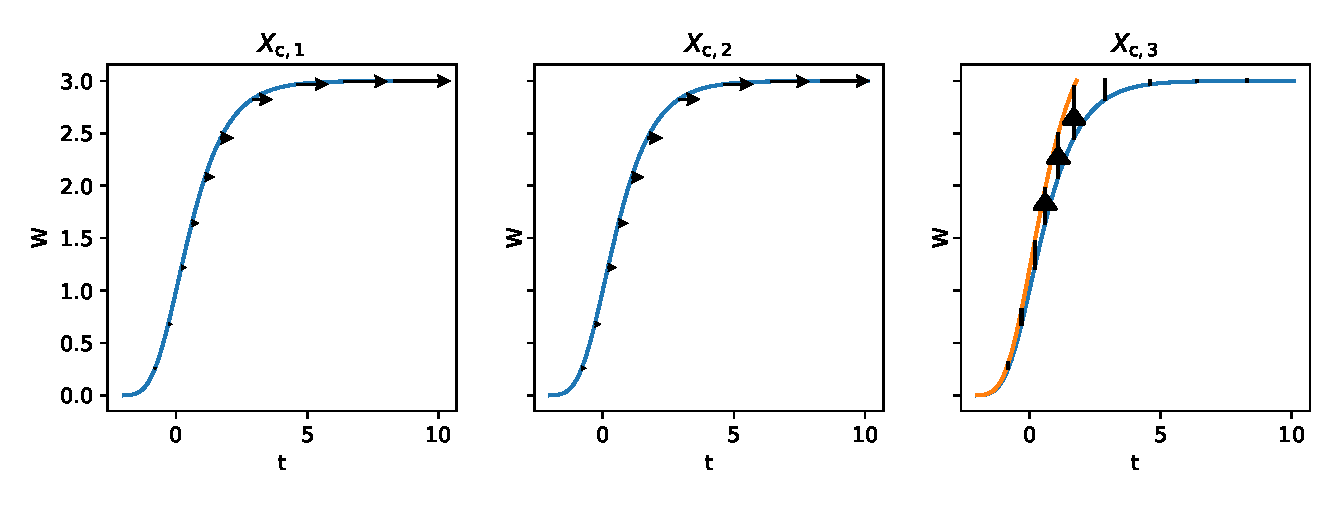
\includegraphics[width=.96\textwidth]{images/gompertz-classical-ansatz}
  \caption{Representative transformations of the Lie groups corresponding to symmetry generators of the classical Gompertz model found using an ansatz.}
  \label{fig:gompertz-classical-ansatz}
\end{figure}

\subsection{The autonomous Gompertz model}

The ansatz
\begin{align*}
  \xi(t, W) &= f_1(t) + f_2(t) \ln(\frac{W}{A}),\\
  \eta(t, W) &= f_3(t) W + f_4(t) \ln(\frac{W}{A}) W
\end{align*}
can be taken, where \(f_i\) for \(i =1,2,3,4\) are arbitrary functions in \(t\).
This results in the determining equation
\begin{align*}
  f_3'(t) W &+ f_4'(t) \ln(\frac{W}{A}) W \\
  &+ \left( f_3(t) + f_4(t) \left( 1 + \ln(\frac{W}{A}) \right) - \left( f_1'(t) + f_2'(t) \ln(\frac{W}{A}) \right) \right) \cdot -k_G \ln(\frac{W}{A}) W \\
  &- \frac{f_2(t)}{W} \left( k_G \ln(\frac{W}{A}) W \right)^2 =\\
  &= \left( f_3(t) W + f_4(t) \ln(\frac{W}{A}) W \right) \cdot -k_G \left( 1 + \ln(\frac{W}{A}) \right)
\end{align*}
which can be reduced to
\begin{align*}
  f_3'(t) W &+ \left( f_4'(t) + k_G f_1'(t) \right) \ln(\frac{W}{A}) W + \left( f_2'(t) - k_G f_2(t) \right) k_G \ln(\frac{W}{A})^2 W =\\
  &= - k_G f_3(t) W
\end{align*}
By separating the equation based on powers of \(\ln(\frac{W}{A})\), the system
\begin{subequations}
  \begin{flalign}
    W & : & f_3'(t) &= -k_G f_3(t) &\label{eq:W}\\
    \ln(\frac{W}{A}) W & : & f_4'(t) + k_G f_1'(t) &= 0 &\label{eq:WA}\\
    k_G \ln(\frac{W}{A})^2 W & : & f_2'(t) - k_G f_2(t) &= 0 &\label{eq:kW2A2W}
  \end{flalign}
\end{subequations}
can be acquired.
This system of equations has the solution
\begin{align*}
  \xi(t, W) &= f_1(t) + c_1 e^{k_G t} \ln(\frac{W}{A}),\\
  \eta(t, W) &= c_2 e^{-k_G t} W + \left( c_3 - k_G f_1(t) \right) \ln(\frac{W}{A}) W,
\end{align*}
where \(c_1\), \(c_2\) and \(c_3\) are arbitrary constants.
Thus, by separating the tangent field into terms with independent arbitrary elements, the infinitesimal generators
\begin{align*}
  X_{\text{a},1} &= e^{k_G t} \ln(\frac{W}{A}) \partial_t \\
  X_{\text{a},2} &= e^{-k_G t} W \partial_W \\
  X_{\text{a},3} &= \ln(\frac{W}{A}) W \partial_W \\
  X_{\text{a},f} &= f(t) \partial_t - k_G f(t) \ln(\frac{W}{A}) W \partial_W
\end{align*}
of Lie point symmetries of the autonomous Gompertz ODE \labelcref{eq:gompertz-autonomous} can be found.
The corresponding transformations can be seen in \cref{fig:gompertz-autonomous-ansatz}.
\begin{figure}
  \centering
  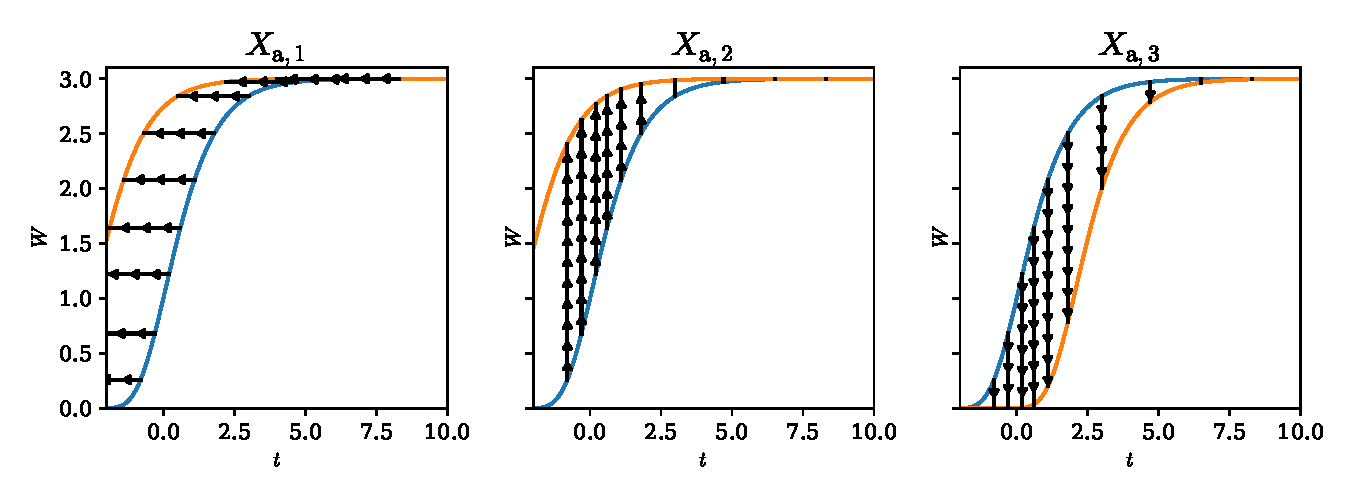
\includegraphics[width=.96\textwidth]{images/gompertz-autonomous-ansatz}
  \caption{Representative transformations of the Lie groups corresponding to symmetry generators of the autonomous Gompertz model found using an ansatz.}
  \label{fig:gompertz-autonomous-ansatz}
\end{figure}

\subsection{The system Gompertz model}

As models and ansätze grow in size, the determining equations grow.
This becomes particularly prominent for systems of ODE:s.
For this reason, the calculations for the remaining models in this chapter have been made using computer algebra using code outlined in \cref{app:computer-algebra}.

Similarly to the classical Gompertz model, the ansatz
\begin{align*}
  \xi{\left(t,W,G \right)} &= \operatorname{f_{1}}{\left(t \right)} + \operatorname{f_{2}}{\left(t \right)} W + \operatorname{f_{3}}{\left(t \right)} G \\
  \eta^{1}{\left(t,W,G \right)} &= \operatorname{f_{4}}{\left(t \right)} + \operatorname{f_{5}}{\left(t \right)} W + \operatorname{f_{6}}{\left(t \right)} G\\
  \eta^{2}{\left(t,W,G \right)} &= \operatorname{f_{7}}{\left(t \right)} + \operatorname{f_{8}}{\left(t \right)} W + \operatorname{f_{9}}{\left(t \right)} G,
\end{align*}
where \(f_i\) are arbitrary functions in \(t\), is used.
The two determining equations can be decomposed in \(W\) and \(G\), resulting in 15 algebraic and ordinary differential equations.
By first solving the algebraic equations, followed by the differential for the arbitrary functions \(f_i\), their form can be determined resulting in the general form
\begin{align*}
  \xi{\left(t,W,G \right)} &= G c_{3} e^{k_{G} t} + c_{1} - \frac{c_{2} e^{k_{G} t}}{k_{G}} \\
  \eta^{1}{\left(t,W,G \right)} &= W c_{4} - \frac{W c_{5} e^{- k_{G} t}}{k_{G}} \\
  \eta^{2}{\left(t,W,G \right)} &= G c_{2} e^{k_{G} t} + c_{5} e^{- k_{G} t}.
\end{align*}
Decomposition in arbitrary constants result in the basis
\begin{align*}
  X_{\text{s},1} &= \partial_t \\
  X_{\text{s},2} &= - \frac{e^{k_{G} t}}{k_{G}} \partial_t + G e^{k_{G} t} \partial_G \\
  X_{\text{s},3} &= G e^{k_{G} t} \partial_t \\
  X_{\text{s},4} &= W \partial_W \\
  X_{\text{s},5} &= - \frac{W e^{- k_{G} t}}{k_{G}} \partial_W + e^{- k_{G} t} \partial_G.
\end{align*}
The corresponding transformations can be seen in \cref{fig:gompertz-system-ansatz}.
\begin{figure}
  \centering
  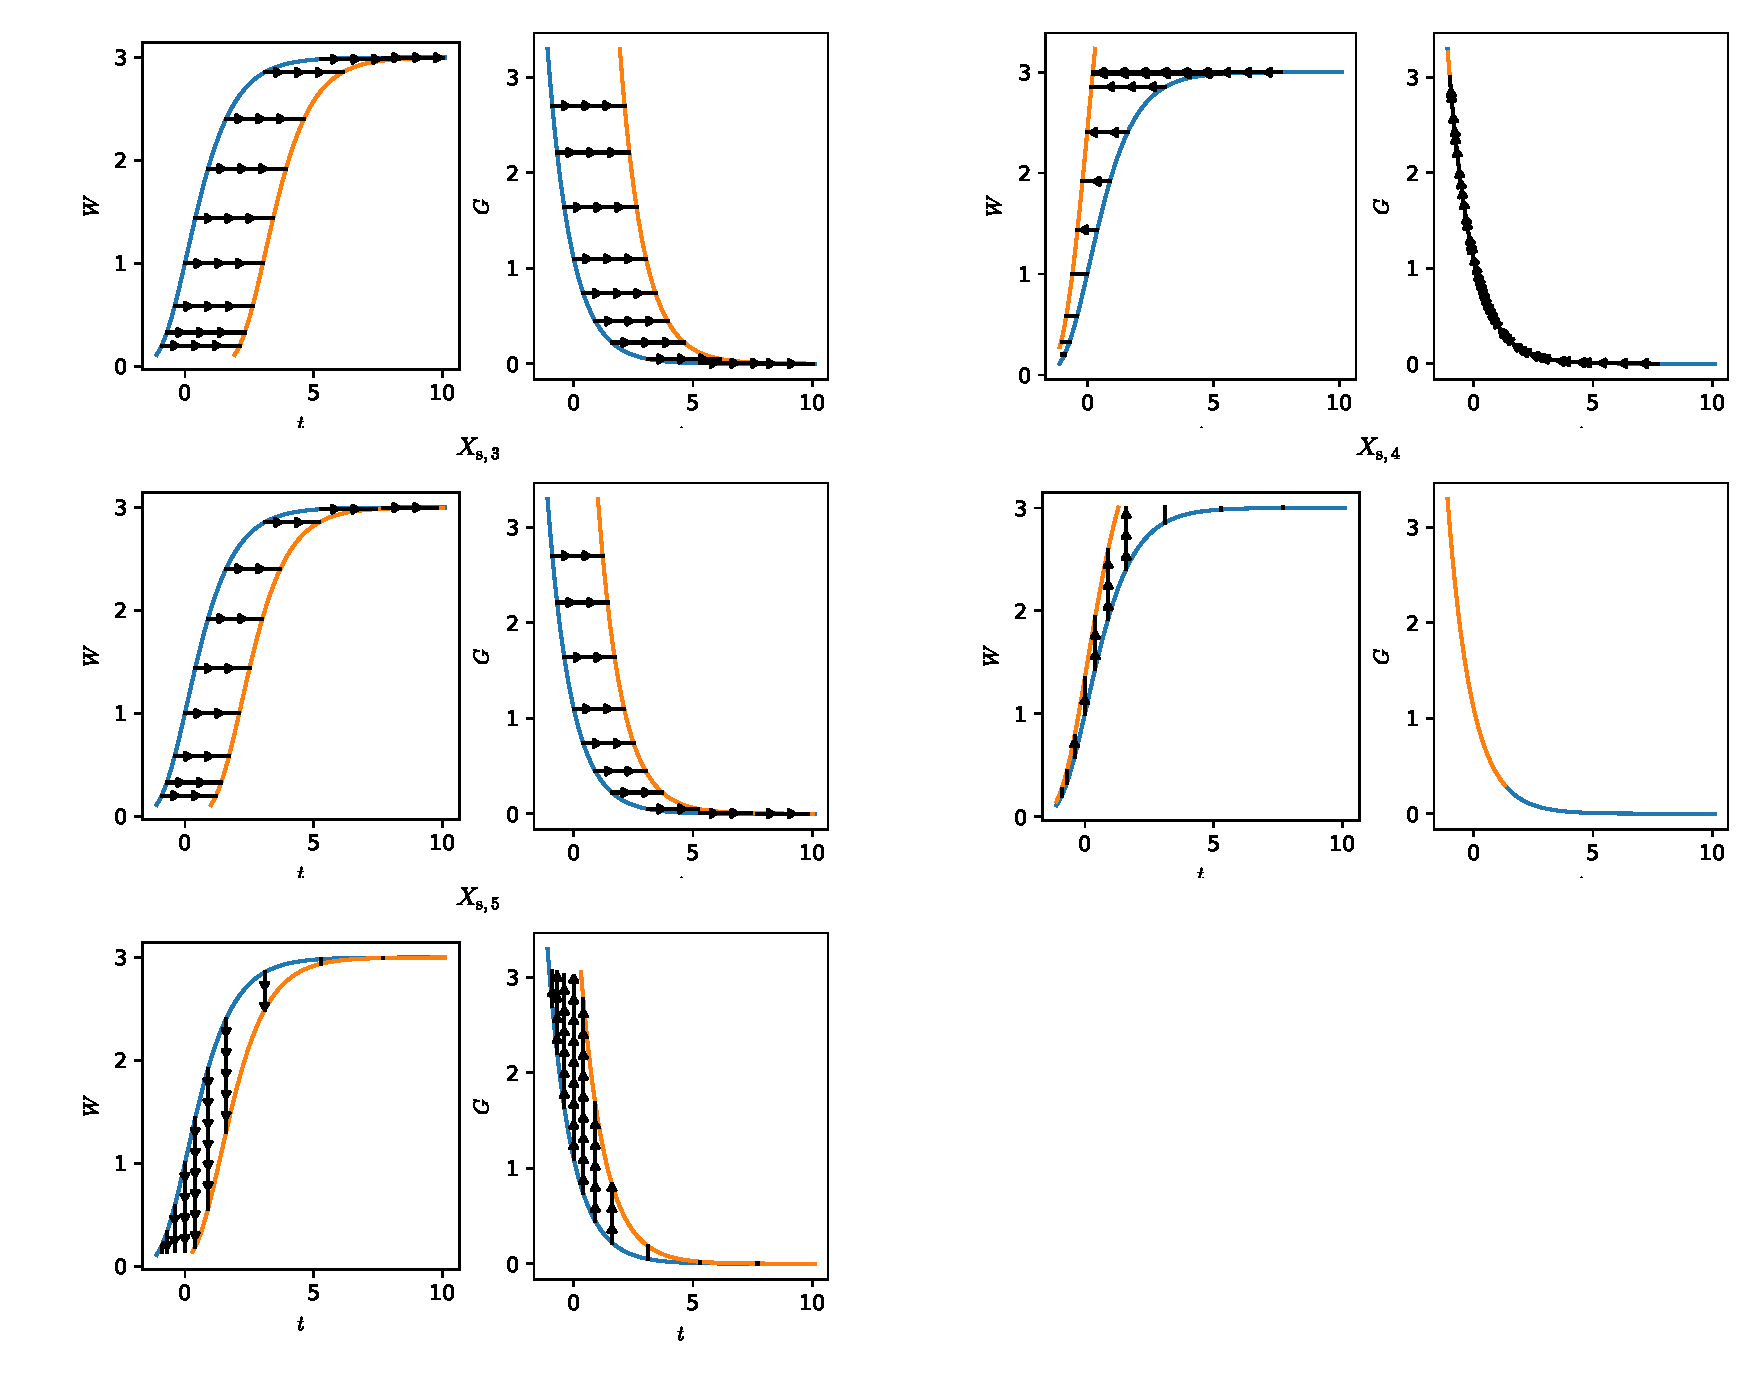
\includegraphics[height=.8\textheight]{images/gompertz-system-ansatz}
  \caption{Representative transformations of the Lie groups corresponding to symmetry generators of the system Gompertz model found using an ansatz.}
  \label{fig:gompertz-system-ansatz}
\end{figure}

\section{The Lotka--Volterra model}

The Lotka--Volterra predator-prey model formulated in \cref{eq:lotka-volterra} has a right hand side formulated as second order polynomial in the two states \(N\) and \(P\).
A good starting point for ansätze is therefore polynomials, and arbitrary third degree polynomials in \(t\), \(N\) and \(P\) are chosen.
The ansatz will thus have the form
\begin{align*}
  \xi &= c_{1,1} + c_{1,2}t + c_{1,3}N + c_{1,4}P + c_{1,5}t^{2} + c_{1,6}tN + c_{1,7}N^{2} + c_{1,8}tP + \\ & \qquad + c_{1,9}NP + c_{1,10}P^{2} + c_{1,11}t^{3} + c_{1,12}t^{2}N + c_{1,13}tN^{2} + c_{1,14}N^{3} + \\ & \qquad + c_{1,15}t^{2}P + c_{1,16}tNP + c_{1,17}N^{2}P + c_{1,18}tP^{2} + c_{1,19}NP^{2} + c_{1,20}P^{3} \\
  \eta^{1} &= c_{2,1} + c_{2,2}t + c_{2,3}N + c_{2,4}P + c_{2,5}t^{2} + c_{2,6}tN + c_{2,7}N^{2} + c_{2,8}tP + \\ & \qquad + c_{2,9}NP + c_{2,10}P^{2} + c_{2,11}t^{3} + c_{2,12}t^{2}N + c_{2,13}tN^{2} + c_{2,14}N^{3} + \\ & \qquad + c_{2,15}t^{2}P + c_{2,16}tNP + c_{2,17}N^{2}P + c_{2,18}tP^{2} + c_{2,19}NP^{2} + c_{2,20}P^{3} \\
  \eta^{2} &= c_{3,1} + c_{3,2}t + c_{3,3}N + c_{3,4}P + c_{3,5}t^{2} + c_{3,6}tN + c_{3,7}N^{2} + c_{3,8}tP + \\ & \qquad + c_{3,9}NP + c_{3,10}P^{2} + c_{3,11}t^{3} + c_{3,12}t^{2}N + c_{3,13}tN^{2} + c_{3,14}N^{3} + \\ & \qquad + c_{3,15}t^{2}P + c_{3,16}tNP + c_{3,17}N^{2}P + c_{3,18}tP^{2} + c_{3,19}NP^{2} + c_{3,20}P^{3},
\end{align*}
where \(c_{i,j}\) are arbitrary constants.
The linearized symmetry condition will thus consist of two equations, each of which must hold for arbitrary \(t\), \(N\) and \(P\).
The two equations can thus be decomposed into 98 linear equations in the arbitrary constants \(c_{i,j}\).
The solution to this overdetermined system of equations gives that any symmetry generator on the form of the ansatz can be written as a linear combination of the generators
\begin{align*}
  X_1 &= \partial_t \\
  X_2 &= \frac{-bNP + aN}{c} \partial_N + \frac{cNP - dP}{c} \partial_P \\
  X_3 &= \frac{t}{c} \partial_t + \frac{-btNP + atN}{c} \partial_N + \frac{ctNP - dtP}{c} \partial_P \\
  X_4 &= \frac{N}{c} \partial_t + \frac{-bcN^2P + acN^2 - bdNP + adN}{c^2} \partial_N + \frac{c^2N^2P - d^2P}{c^2} \partial_P \\
  X_5 &= \frac{P}{c} \partial_t + \frac{-bNP^2 + aNP}{c} \partial_N + \frac{cNP^2 - dP^2}{c} \partial_P
\end{align*}

\section{The Yildirim--Mackey lactose operon model}

Since the lactose operon model formulated in \cref{eq:lac-operon} is significantly larger than all other models studied, the performance of the computer algebra system places restrictions on the ansätze viable to test.
Additionally, the decomposition of the linearized symmetry condition becomes less straight forward as the right hand side of the lactose operon model contains both fractions and arbitrary powers of the state \(A\).

A simple ansatz is that the infinitesimal generator is linear in time and the states, formulated as
\begin{align*}
  \xi &= c_{1,1} + c_{1,2}t + c_{1,3}M + c_{1,4}B + c_{1,5}L + c_{1,6}A + c_{1,7}P \\
  \eta^{1} &= c_{2,1} + c_{2,2}t + c_{2,3}M + c_{2,4}B + c_{2,5}L + c_{2,6}A + c_{2,7}P \\
  \eta^{2} &= c_{3,1} + c_{3,2}t + c_{3,3}M + c_{3,4}B + c_{3,5}L + c_{3,6}A + c_{3,7}P \\
  \eta^{3} &= c_{4,1} + c_{4,2}t + c_{4,3}M + c_{4,4}B + c_{4,5}L + c_{4,6}A + c_{4,7}P \\
  \eta^{4} &= c_{5,1} + c_{5,2}t + c_{5,3}M + c_{5,4}B + c_{5,5}L + c_{5,6}A + c_{5,7}P \\
  \eta^{5} &= c_{6,1} + c_{6,2}t + c_{6,3}M + c_{6,4}B + c_{6,5}L + c_{6,6}A + c_{6,7}P,
\end{align*}
where  \(c_{i,j}\) are arbitrary constants.
The linearized symmetry condition will thus consist of 5 equations, which will consist of sums of fractional expressions in the states.
To decompose the system, the sums in all equations are rewritten with a common denominator.
Additionally, since the power \(A^n\) appear in some of the equations, and all equations sought should hold for an arbitrary \(n\), the numerator of the equations written with common denominators is decomposed in \(t\), \(M\), \(B\), \(L\), \(A\) \(P\) and \(A^n\).
The decomposition results in 1901 equations, all linear in the arbitrary constants \(c_{i,j}\).
The solution to the overdetermined system of equations gives that the only symmetry generator on the form of the ansatz is the manifest generator
\begin{equation*}
  X_1 = \partial_t.
\end{equation*}


\chapter{Finding symmetries using parameter independence}\label{ch:param-ind}

In \cref{ch:ansatze} the traditional approach of using ansätze to find symmetries of first order ODE:s was used.
There are two main problems with using ansätze.

Firstly, there is a lack of systematics in the process.
There are algorithms that have high success rates at finding symmetries of first order ODE:s that use a heuristic approach \cite{chebterrab1997computer,chebterrab1998patterns}.
These methods are however not aimed at finding as many symmetries as possible, but rather finding enough symmetries to integrate the system.
If the goal is to draw new biological conclusions from the symmetries, this is insufficient, as the algorithm is considered equally good if it finds the time invariance generated by \(\partial_t\) as if it finds a more biologically complex symmetry.
Thus such schemes would have to be reevaluated, focusing on metrics such as the number of symmetries, and run on collections of ODE:s on forms common in biology.

Secondly, using ansätze to find symmetries gives information about systems unreliably.
Unless the ansatz can be tied to some biological concept independently of the system studied, solving the symmetry conditions using an ansatz only contributes to the knowledge about the systems if new symmetries are found.
Any negative information about which symmetries exist will be hard enough to interpret that it will be discarded in most cases.

In this chapter, a new approach to making the linearized symmetry condition viable to solve for first order ODE:s is presented and used.
The central concept of the method is finding symmetries that are independent of one or more parameters of an ODE model.
It is heavily inspired by methods used in group classification introduced by \citeauthor{ovsiannikov1982group} \cite{ovsiannikov1982group}.
The group classification problem centers around models that contain parameters which are not limited to being constants, but instead can be any arbitrary function in the states of the model.
The general biological models described in \cref{ch:models} are special cases of such models, where the parameters are limited to being constants.
This chapter has a description of the method of parameter independence for such models, followed by application of the method to the models under study.

\section{The parameter independence method}

Consider a system of first order ODE:s
\begin{equation} \label[ode]{eq:generic-param-ode}
  \diff{\vect{u}}{t} = \vect{\omega}(t, \vect{u}; \vect{\theta})
\end{equation}
with states \(\vect{u} = \left(u^1, \dots, u^s\right)\), parametrized by constant parameters \(\vect{\theta} = \left(\theta^1, \dots, \theta^m\right)\).
In traditional symmetry calculations, \cref{eq:generic-param-ode} is seen as a single equation, where the parameters \(\vect{\theta}\) have unknown but fixed values.
Any symmetry found through calculations is a symmetry of the equation defined by that specific set of parameters \(\vect{\theta}\), which shows itself in symmetry generators themselves containing the parameters.
In contrast, an ODE used in modeling is often seen as a collection of models.
Some parameters might be fixed at the same value in all valid uses of the model, but most parameters are intended to vary over different use cases.
To take biochemistry as an example, while some parameters might indicate the reaction speed between two chemicals (which is seen as fixed), most parameters are intended to vary between conditions the cells are in or between individuals in a cell population.

When interpreting symmetries, the distinction between symmetries for specific instances of the model and symmetries of certain families of the model becomes important.
While there are no known methods for finding all the symmetries of a specific system of first order ODE:s, it is possible to find all symmetries common to a family parametrized by one of the parameters \(\theta^1, \dots, \theta^m\).
Without loss of generality, the one-parameter family of functions
\begin{equation*} %\label{eq:generic-param-family}
  \Omega = \left\{\vect{u}_t - \vect{\omega}(t, \vect{u}; \vect{\theta}):\quad \theta^1 \in S \subseteq \reals \right\}
\end{equation*}
with fixed parameters \(\theta^2, \dots, \theta^m\) can be considered.
Call a Lie point symmetry with infinitesimal generator \(X = \xi(x, \vect{u}) \partial_t + \vect{\eta}(x, \vect{u}) \cdot \partial_{\vect{u}}\) a symmetry of the family of ODE:s defined by
\begin{equation*}
  \vect{\Delta}(\prolong{z}{1}) = 0 ,\quad \vect{\Delta} \in \Omega
\end{equation*}
if
\begin{equation*}
  \eval{\prolong{X}{1}\left(\vect{\Delta}(\prolong{z}{1})\right)}_{\vect{\Delta}(\prolong{z}{1}) = 0} = 0 ,\quad \forall \vect{\Delta} \in \Omega.
\end{equation*}
Thus, an infinitesimal generator \(X\) of a family of ODE:s defined by \(\Omega\) can not have any dependence on \(\theta^1\).
Evaluating the linearized symmetry condition, it takes the form
\begin{equation*}
  \eta_t - \omega^k \xi_t + \sum_{i=1}^s \omega^i \eta^k_{u^i} - \sum_{i=1}^s \omega^k \omega^i \xi_{u^i} -
  \omega^k_t \xi - \sum_{i=1}^s \omega^k_{u^i} \eta^i = 0 ,\quad \forall k = 1, \dots, s.
\end{equation*}
Since the parameter \(\theta^1\) appears in at least one function \(\omega^j\), and every equation of the linearized symmetry condition includes any \(\omega^j\) at least once, decomposition of the equations in \(\theta^1\) results in a set of at least \(2 s + 1\) equations (taking the \(\omega^k \omega^k\)-term for equation \(k = j\) into account), that will henceforth be called the parameter independence determining equations.
Just like the determining equations for higher order ODE:s, the parameter independence determining equations create a solvable system of PDE:s, whose solution is the most general form of a symmetry generator for the problem.

This method addresses both previously mentioned weaknesses of using ansätze.
Firstly, the process of finding symmetries by parameter independence is highly systematic.
The method can be used for all parameters of a model, at which point calculations will have revealed all Lie point symmetries independent of one or more of the parameters of the model.
This creates a clear stopping point for calculations.
Secondly, calculations resulting in no parameter independent symmetries being found can still be informative to the modeler since most parameters tend to be connected to some natural concept.

\section{The Gompertz model}
To reiterate, the Gompertz models are\par\noindent
\begin{tabularx}{\linewidth}{rrM}
  Classical, & \(T_i\) :&
  \begin{minipage}{\linewidth}
    \begin{equation}
      \diff{W}{t} = k_G e^{-k_G (t - T_i)} W(t) \label{eq:gompertz-classical-ti^param}
    \end{equation}
  \end{minipage}\tabularnewline
  Classical, & \(W_0\) :&
  \begin{minipage}{\linewidth}
    \begin{equation}
      \diff{W}{t} = k_G \ln\left(\frac{W_0}{A}\right)e^{-k_G t} W(t) \label{eq:gompertz-classical-w0^param}
    \end{equation}
  \end{minipage}\tabularnewline
  Autonomous, & \(T_i\) and \(W_0\) :&
  \begin{minipage}{\linewidth}
    \begin{equation}
      \diff{W}{t} = -k_G \ln\left(\frac{W(t)}{A}\right) W(t) \label{eq:gompertz-autonomous^param}
    \end{equation}
  \end{minipage}\tabularnewline
  System, & \(T_i\) and \(W_0\) :&
  \begin{minipage}{\linewidth}%
    {\begin{subequations} \label[subequations]{eq:gompertz-system^param}
      \begin{align}
        \diff{W}{t} &= G(t) W(t) \label{eq:gompertz-system-a^param}\\
        \diff{G}{t} &= -k_G G(t). \label{eq:gompertz-system-b^param}
      \end{align}
    \end{subequations}}%
  \end{minipage}
\end{tabularx}
As was seen in \cref{ch:ansatze}, several symmetries exist for each of the models.
Some of these symmetries were independent of one or more parameters, and should therefore be found using the parameter independence method.
It is however of interest to see if any symmetries not found using the specific ansätze used in \cref{ch:ansatze} can be found using the parameter independence method.

\subsection{The classical Gompertz model}

For the classical Gompertz model, two different parametrizations exist.
For the purposes of the parameter independence method, either of these parametrizations may be used since the parameters \(T_i\) and \(W_0\) only depend on each other and the parameter \(k_G\), but neither the time \(t\) nor the state \(W\).
The \(T_i\)-parametrization will be used in these calculations.

The linearized symmetry condition \labelcref{eq:linearized-first-order-symmetry} is for the classical \(T_i\)-parametrized Gompertz model
\begin{equation}\label{eq:gompertz-classical-lin-symmetry-cond}
  \begin{split}
    \eta_t &+ k_G e^{-k_G (t - T_i)} W\left(\eta_W - \xi_t\right) - (k_G)^2 e^{-2k_G (t - T_i)} W^2 \xi_W +\\ &+ (k_G)^2 e^{-k_G (t - T_i)} W \xi - k_G e^{-k_G (t - T_i)} \eta = 0.
  \end{split}
\end{equation}
For a generator \(\left(\xi, \eta\right)\) to be independent of a parameter, \cref{eq:gompertz-classical-lin-symmetry-cond} is decomposed by functionally independent coefficients of that parameter.

\subsubsection{\texorpdfstring{\(k_G\)-independent symmetries}{Growth rate-independent symmetries}}

Decomposition of \cref{eq:gompertz-classical-lin-symmetry-cond} in \(k_G\) gives the parameter independence determining equations
\begin{subequations}
  \begin{flalign}
    1 & : & \eta_t &= 0 &\label{eq:gompertz-classical-det-kg-a}\\
    k_G e^{-k_G (t - T_i)} & : & W \left(\eta_W - \xi_t\right) - \eta &= 0 &\label{eq:gompertz-classical-det-kg-b}\\
    (k_G)^2 e^{-k_G (t - T_i)} & : & W \xi &= 0 &\label{eq:gompertz-classical-det-kg-c}\\
    (k_G)^2 e^{-2k_G (t - T_i)} & : & W^2 \xi_W &= 0. &\label{eq:gompertz-classical-det-kg-d}
  \end{flalign}
\end{subequations}
From \cref{eq:gompertz-classical-det-kg-c} it is clear that
\begin{equation*}
  \xi \equiv 0,
\end{equation*}
and hence \cref{eq:gompertz-classical-det-kg-d} must also hold.
From \cref{eq:gompertz-classical-det-kg-a} it is clear that
\begin{equation*}
  \eta = \eta(W)
\end{equation*}
is a function only in \(W\).
This leaves \cref{eq:gompertz-classical-det-kg-b} that simplifies into the ODE
\begin{equation*}
  W \eta_W - \eta = 0
\end{equation*}
with the general solution
\begin{equation*}
  \eta = c_1 W,
\end{equation*}
where \(c_1\) is an arbitrary constant.
Thus any \(k_G\)-independent symmetry generator of the classical Gompertz model \labelcref{eq:gompertz-classical-ti^param} must have the form
\begin{align*}
  \xi &= 0 \\
  \eta &= c_1 W,
\end{align*}
which is spanned by the generator basis
\begin{equation*}
  X_{\text{c},4} = W \partial_W.
\end{equation*}

\subsubsection{\texorpdfstring{\(T_i\)-independent symmetries}{Inflection time-independent symmetries}}

Decomposition of \cref{eq:gompertz-classical-lin-symmetry-cond} in \(T_i\) gives the parameter independence determining equations
\begin{subequations}
  \begin{flalign}
    1 & : & \eta_t &= 0 &\label{eq:gompertz-classical-det-ti-a}\\
    e^{k_G T_i} & : & k_G e^{-k_G t} W \left(\eta_W - \xi_t\right) + (k_G)^2 e^{-k_G t} W \xi - k_G e^{-k_G t} \eta &= 0 &\label{eq:gompertz-classical-det-ti-b}\\
    e^{2 k_G T_i} & : & -(k_G)^2 e^{-2 k_G t} W^2 \xi_W &= 0 &\label{eq:gompertz-classical-det-ti-c}
  \end{flalign}
\end{subequations}
From \cref{eq:gompertz-classical-det-ti-a,eq:gompertz-classical-det-ti-c} it is clear that
\begin{align*}
  \eta &= \eta(W) \\
  \xi &= \xi(t)
\end{align*}
respectively.
Dividing \cref{eq:gompertz-classical-det-ti-b} by \(k_G e^{-k_G t}\) gives
\begin{equation}\label{eq:gompertz-classical-det-ti-b-simple}
  W \left(\eta_W - \xi_t\right) + k_G W \xi - \eta = 0,
\end{equation}
which can be rewritten as
\begin{equation}
  k_G \xi - \xi_t = \frac{\eta}{W} - \eta_W.
\end{equation}
Separation of variables gives that
\begin{equation}
  k_G \xi - \xi_t = c_1 = \frac{\eta}{W} - \eta_W
\end{equation}
for some constant \(c_1\), where both the left and right hand sides are straight forward to solve since they are only dependent in one variable each.
Thus any \(T_i\)-independent symmetry generator of the classical Gompertz model \labelcref{eq:gompertz-classical-ti^param} must have the form
\begin{align*}
  \xi &= \frac{c_1}{k_G} + c_2 e^{k_G t} \\
  \eta &= -c_1 W \ln\left(W\right) + c_3 W,
\end{align*}
which is spanned by the generator basis
\begin{align*}
  X_{\text{c},1} &= e^{k_G t} \partial_t \\
  X_{\text{c},4} &= W \partial_W \\
  X_{\text{c},5} &= \partial_t - k_G W \ln\left(W\right) \partial_W.
\end{align*}

\subsubsection{All of the found generators}
The basis of all the generators found by the parameter independence method for the classical Gompertz model are
\begin{align*}
  X_{\text{c},1} &= e^{k_G t} \partial_t \\
  X_{\text{c},4} &= W \partial_W \\
  X_{\text{c},5} &= \partial_t - k_G W \ln\left(W\right) \partial_W.
\end{align*}
The corresponding transformations can be seen in \cref{fig:gompertz-classical-param}.
\begin{figure}
  \centering
  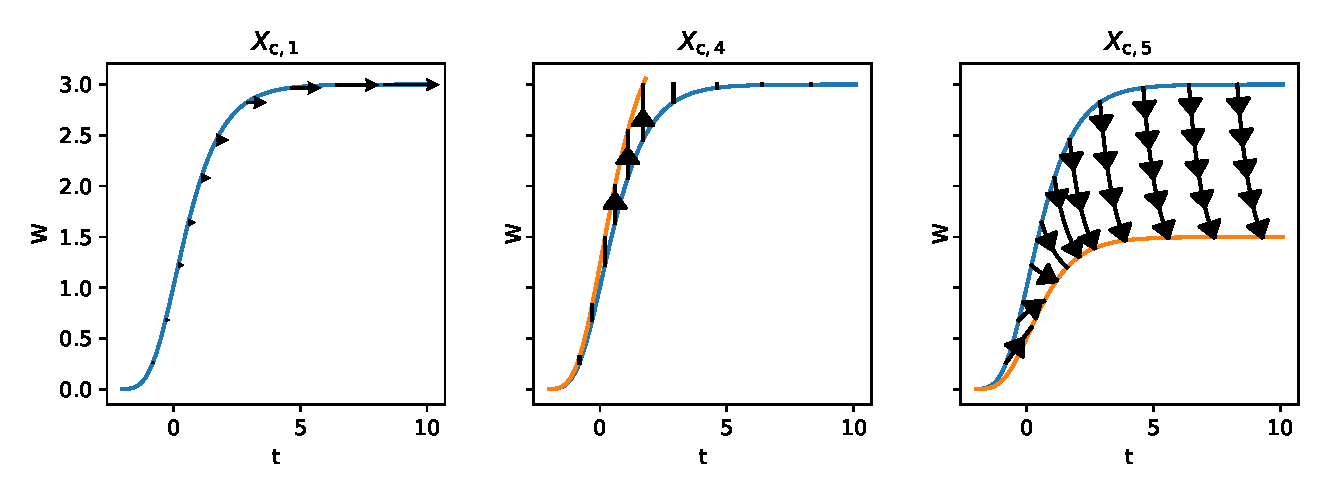
\includegraphics[width=.6517\textwidth]{images/gompertz-classical-param}
  \caption{
    Representative transformations of the Lie groups corresponding to symmetry generators of the classical Gompertz model found using the parameter independence method.
    For the generator \(X_{\text{c},1}\), a vector field is instead shown since the symmetry generator only acts locally.
    The \(\dl t\)-- and \(\dl W\)--components of the vector field is shown on a \(\log(1 + x)\) scale.
  }
  \label{fig:gompertz-classical-param}
\end{figure}


\subsection{The autonomous Gompertz model}

For the autonomous Gompertz model there is only one parametrization of interest.
The linearized symmetry condition \labelcref{eq:linearized-first-order-symmetry} is for the autonomous Gompertz model
\begin{equation}\label{eq:gompertz-autonomous-lin-symmetry-cond}
  \begin{split}
    \eta_t &- k_G \ln\left(\frac{W}{A}\right) W\left(\eta_W - \xi_t\right) - (k_G)^2 \left(\ln\left(\frac{W(t)}{A}\right)\right)^2 W^2 \xi_W +\\ &+ k_G \left(\ln\left(\frac{W}{A}\right) + 1\right) \eta = 0.
  \end{split}
\end{equation}

\subsubsection{\texorpdfstring{\(k_G\)-independent symmetries}{Growth rate-independent symmetries}}

Decomposition of \cref{eq:gompertz-autonomous-lin-symmetry-cond} in \(k_G\) gives the parameter independence determining equations
\begin{subequations}
  \begin{flalign}
    1 & : & \eta_t &= 0 &\label{eq:gompertz-autonomous-det-kg-a}\\
    k_G & : & -\ln\left(\frac{W}{A}\right) W\left(\eta_W - \xi_t\right) + \left(\ln\left(\frac{W}{A}\right) + 1\right) \eta &= 0 &\label{eq:gompertz-autonomous-det-kg-b}\\
    (k_G)^2 & : & -\left(\ln\left(\frac{W(t)}{A}\right)\right)^2 W^2 \xi_W &= 0. &\label{eq:gompertz-autonomous-det-kg-c}
  \end{flalign}
\end{subequations}
From \cref{eq:gompertz-autonomous-det-kg-a,eq:gompertz-autonomous-det-kg-c}
\begin{align*}
  \eta &= \eta(W) \\
  \xi &= \xi(t).
\end{align*}
Hence, since the only source of time dependence in \cref{eq:gompertz-autonomous-det-kg-b} is \(\xi_t\),
\begin{equation*}
  \xi_t = c_1
\end{equation*}
where \(c_1\) is an arbitrary constant, and thus
\begin{equation*}
  \xi = c_1 t + c_2
\end{equation*}
for an additional arbitrary constant \(c_2\).
\Cref{eq:gompertz-autonomous-det-kg-b} can thus be rewritten as
\begin{equation*}
  \eta_W - \frac{\ln\left(\frac{W}{A}\right) + 1}{\ln\left(\frac{W}{A}\right) W} \eta - c_1 = 0,
\end{equation*}
which is a scalar first order ODE with the solution
\begin{equation*}
  \eta = c_1 \ln\left(\abs{\ln\left(\frac{W}{A}\right)}\right) \ln\left(\frac{W}{A}\right) W + c_3 \ln\left(\frac{W}{A}\right) W.
\end{equation*}
Thus any \(k_G\)-independent symmetry generator of the autonomous Gompertz model \labelcref{eq:gompertz-autonomous^param} must have the form
\begin{align*}
  \xi &= c_2 + c_1 t \\
  \eta &= c_1 \ln\left(\abs{\ln\left(\frac{W}{A}\right)}\right) \ln\left(\frac{W}{A}\right) W + c_3 \ln\left(\frac{W}{A}\right) W,
\end{align*}
which is spanned by the generator basis
\begin{align*}
  X_{\text{a},3} &= \ln\left(\frac{W}{A}\right) W \partial_W \\
  X_{\text{a},4} &= \partial_t \\
  X_{\text{a},5} &= t \partial_t + \ln\left(\abs{\ln\left(\frac{W}{A}\right)}\right) \ln\left(\frac{W}{A}\right) W \partial_W.
\end{align*}

\subsubsection{\texorpdfstring{\(A\)-independent symmetries}{Carrying capacity-independent symmetries}}

Decomposition of \cref{eq:gompertz-autonomous-lin-symmetry-cond} in \(A\) gives the parameter independence determining equations
\begin{subequations}
  \begin{flalign}
    1 & : & \eta_t + k_G \eta &= 0 &\label{eq:gompertz-autonomous-det-a-a}\\
    \ln\left(\frac{W}{A}\right) & : & - k_G W\left(\eta_W - \xi_t\right)  + k_G \eta &= 0 &\label{eq:gompertz-autonomous-det-a-b}\\
    \left(\ln\left(\frac{W}{A}\right)\right)^2 & : & - (k_G)^2 W^2 \xi_W &= 0. &\label{eq:gompertz-autonomous-det-a-c}
  \end{flalign}
\end{subequations}
From \cref{eq:gompertz-autonomous-det-a-c}
\begin{equation*}
  \xi = \xi(t).
\end{equation*}
Since \(\eta\) (and thus its derivative) are the only unknown sources of \(W\)-dependence in \cref{eq:gompertz-autonomous-det-a-b},
\begin{equation*}
  \eta_W - \frac{1}{W}\eta = \xi_t(t)
\end{equation*}
must hold.
Integration in \(W\) gives
\begin{equation*}
  \eta = \ln\left(W\right) W \xi_t(t) + W f(t)
\end{equation*}
for some arbitrary function \(f\) in time.
Inserting this result in \cref{eq:gompertz-autonomous-det-a-a} gives
\begin{equation*}
  \ln\left(W\right) W \xi_{tt} + W f_t + k_G \ln\left(W\right) W \xi_t + k_G W f = 0
\end{equation*}
which can be decomposed by \(W\) into
\begin{align*}
  \xi_{tt} + k_G \xi_t &= 0 \\
  f_t + k_G f &= 0
\end{align*}
with solutions
\begin{align*}
  \xi &= - c_1 \frac{1}{k_G} e^{-k_G t} + c_2 \\
  f &= c_3 e^{-k_G t}.
\end{align*}
Thus any \(A\)-independent symmetry generator of the autonomous Gompertz model \labelcref{eq:gompertz-autonomous^param} must have the form
\begin{align*}
  \xi &= - c_1 \frac{1}{k_G} e^{-k_G t} + c_2 \\
  \eta &= c_1 e^{-k_G t} \ln\left(W\right) W  + c_3 e^{-k_G t} W,
\end{align*}
which is spanned by the generator basis
\begin{align*}
  X_{\text{a},2} &= e^{-k_G t} W \partial_W \\
  X_{\text{a},4} &= \partial_t \\
  X_{\text{a},6} &= e^{-k_G t} \partial_t - k_G e^{-k_G t} \ln\left(W\right) W \partial_W.
\end{align*}

\subsubsection{All found generators}
The basis of all the generators found by the parameter independence method for the autonomous Gompertz model are
\begin{align*}
  X_{\text{a},2} &= e^{-k_G t} W \partial_W \\
  X_{\text{a},3} &= \ln\left(\frac{W}{A}\right) W \partial_W \\
  X_{\text{a},4} &= \partial_t \\
  X_{\text{a},5} &= t \partial_t + \ln\left(\abs{\ln\left(\frac{W}{A}\right)}\right) \ln\left(\frac{W}{A}\right) W \partial_W \\
  X_{\text{a},6} &= e^{-k_G t} \partial_t - k_G e^{-k_G t} \ln\left(W\right) W \partial_W.
\end{align*}
The corresponding transformations can be seen in \cref{fig:gompertz-autonomous-param}.
\begin{figure}
  \centering
  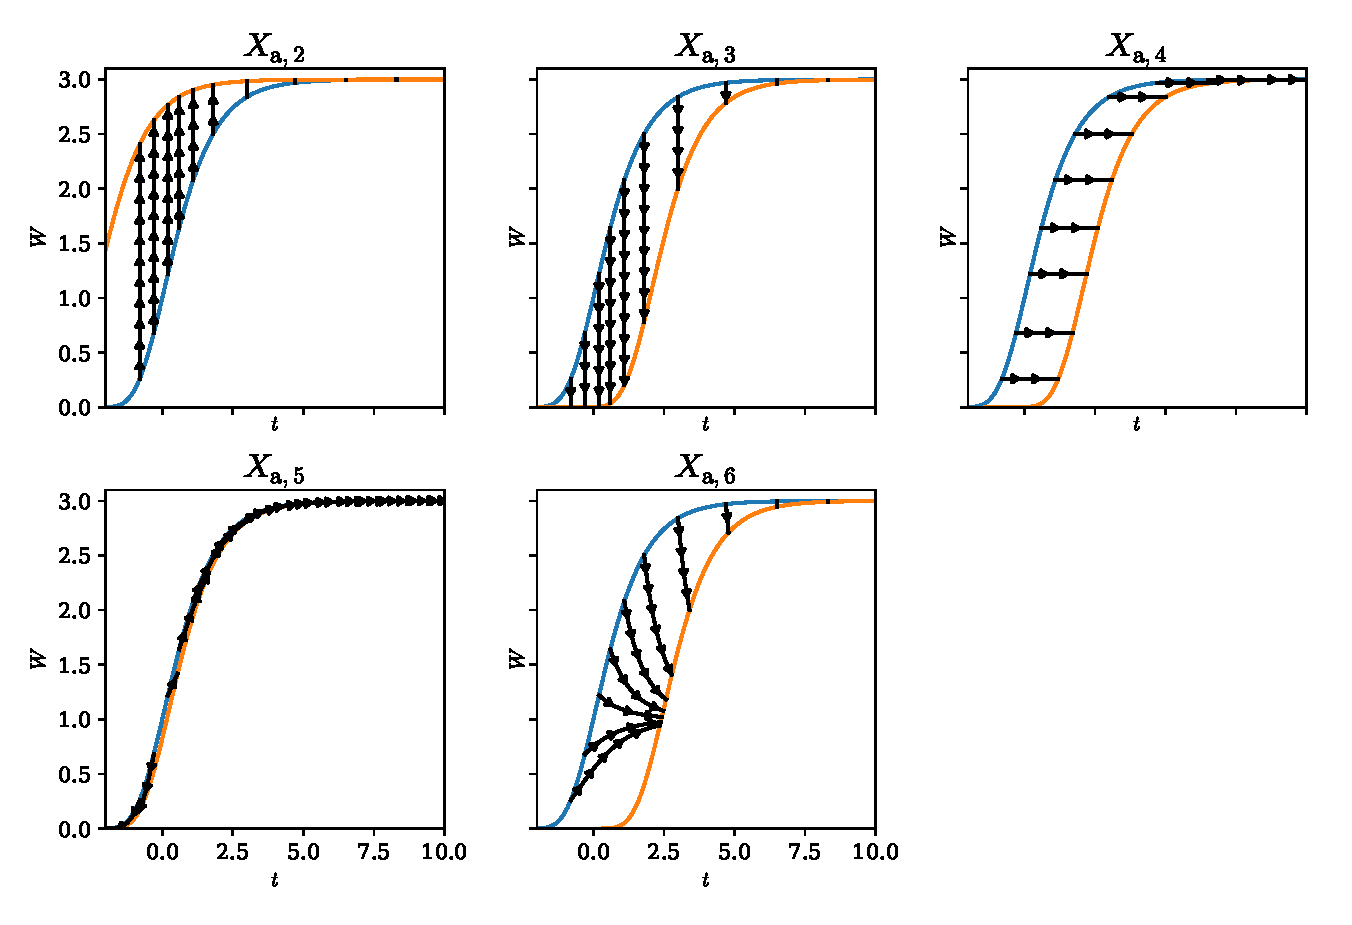
\includegraphics[width=.96\textwidth]{images/gompertz-autonomous-param}
  \caption{Representative transformations of the Lie groups corresponding to symmetry generators of the autonomous Gompertz model found using the parameter independence method.}
  \label{fig:gompertz-autonomous-param}
\end{figure}

\subsection{The system Gompertz model}

For the system Gompertz model there is also only one parametrization of interest.
The linearized symmetry condition \labelcref{eq:linearized-first-order-symmetry} is for the system Gompertz model
\begin{subequations} \label[subequations]{eq:gompertz-system-lin-symmetry-cond}
  \begin{align}
    \begin{split}\label{eq:gompertz-system-lin-symmetry-cond-a}
      \eta^1_t + W G \left(\eta^1_W - \xi_t\right) -k_G G \eta^1_G - W^2 G^2 \xi_W +&\\+ k_G W G^2 \xi_G - G \eta^1 - W \eta^2 &= 0 
    \end{split}\\
    \begin{split}\label{eq:gompertz-system-lin-symmetry-cond-b}
      \eta^2_t - k_G G \left(\eta^2_G - \xi_t\right) + W G \eta^2_W + k_G W G^2 \xi_W -&\\- (k_G)^2 G^2 \xi_G + k_G \eta^2 &= 0. 
    \end{split}
  \end{align}
\end{subequations}

\subsubsection{\texorpdfstring{\(k_G\)-independent symmetries}{Growth rate-independent symmetries}}

Decomposition of \cref{eq:gompertz-system-lin-symmetry-cond} in \(k_G\) gives the parameter independence determining equations
\begin{subequations}
  \begin{flalign}
    \labelcref{eq:gompertz-system-lin-symmetry-cond-a},\ & 1 : & \eta^1_t + W G \left(\eta^1_W - \xi_t\right) - W^2 G^2 \xi_W - G \eta^1 - W \eta^2 &= 0 &\label{eq:gompertz-system-det-kg-a}\\
    \labelcref{eq:gompertz-system-lin-symmetry-cond-a},\ & k_G : & - G \eta^1_G + W G^2 \xi_G &= 0 &\label{eq:gompertz-system-det-kg-b}\\
    \labelcref{eq:gompertz-system-lin-symmetry-cond-b},\ & 1 : & \eta^2_t + W G \eta^2_W &= 0. &\label{eq:gompertz-system-det-kg-c} \\
    \labelcref{eq:gompertz-system-lin-symmetry-cond-b},\ & k_G : & - G \left(\eta^2_G - \xi_t\right) + W G^2 \xi_W + \eta^2 &= 0. &\label{eq:gompertz-system-det-kg-d} \\
    \labelcref{eq:gompertz-system-lin-symmetry-cond-b},\ & (k_G)^2 : & - G^2 \xi_G &= 0. &\label{eq:gompertz-system-det-kg-e}
  \end{flalign}
\end{subequations}
From \cref{eq:gompertz-system-det-kg-e} it is clear that
\begin{equation} \label{eq:system-gompertz-kG-first-simplification-1}
  \xi = \xi(t, W),
\end{equation}
and thus from \cref{eq:gompertz-system-det-kg-b}
\begin{equation} \label{eq:system-gompertz-kG-first-simplification-2}
  \eta^1 = \eta^1(t, W).
\end{equation}
From \cref{eq:gompertz-system-det-kg-a}
\begin{equation*}
  \eta^2 = \frac{1}{W}\eta^1_t + G \left(\eta^1_W - \xi_t - \frac{1}{W} \eta^1 \right) - W G^2 \xi_W,
\end{equation*}
and thus \cref{eq:gompertz-system-det-kg-d} can be written as
\begin{equation}\label{eq:gompertz-system-det-kg-d-simple}
  \frac{1}{W}\eta^1_t + G \xi_t + 2 G^2 W \xi_W = 0.
\end{equation}
Since both \(\xi\) and \(\eta^1\) are not functions in \(G\), \cref{eq:gompertz-system-det-kg-d-simple} can be decomposed in \(G\) giving
\begin{align*}
  \xi_t &= 0 \\
  \xi_W &= 0 \\
  \eta^1_t &= 0.
\end{align*}
Thus
\begin{align*}
  \xi &= c_1 \\
  \eta^1 &= \eta^1(W) \\
  \eta^2 &= G \left(\eta^1_W(W) - \frac{1}{W} \eta^1(W) \right),
\end{align*}
where \(c_1\) is an arbitrary constant, and \cref{eq:gompertz-system-det-kg-c} reduces to
\begin{equation*}
  W G^2 \left(\eta^1_W - \frac{1}{W} \eta^1 \right)_W = 0.
\end{equation*}
Thus the ODE
\begin{equation*}
  \eta^1_W - \frac{1}{W} \eta^1 = c_2
\end{equation*}
must hold for an arbitrary constant \(c_2\), which has the general solution
\begin{equation*}
  \eta^1 = c_2 \ln\left(W\right) W + c_3 W.
\end{equation*}
Thus any \(k_G\)-independent symmetry generator of the system Gompertz model \labelcref{eq:gompertz-system^param} must have the form
\begin{align*}
  \xi &= c_1 \\
  \eta^1 &= c_2 \ln\left(W\right) W + c_3 W\\
  \eta^2 &= c_2 G
\end{align*}
which is spanned by the generator basis
\begin{align*}
  X_{\text{s},1} &= \partial_t \\
  X_{\text{s},4} &= W \partial_W \\
  X_{\text{s},6} &= \ln\left(W\right) W \partial_W + G \partial_G.
\end{align*}
The corresponding transformations can be seen in \cref{fig:gompertz-system-param}.
\begin{figure}
  \centering
  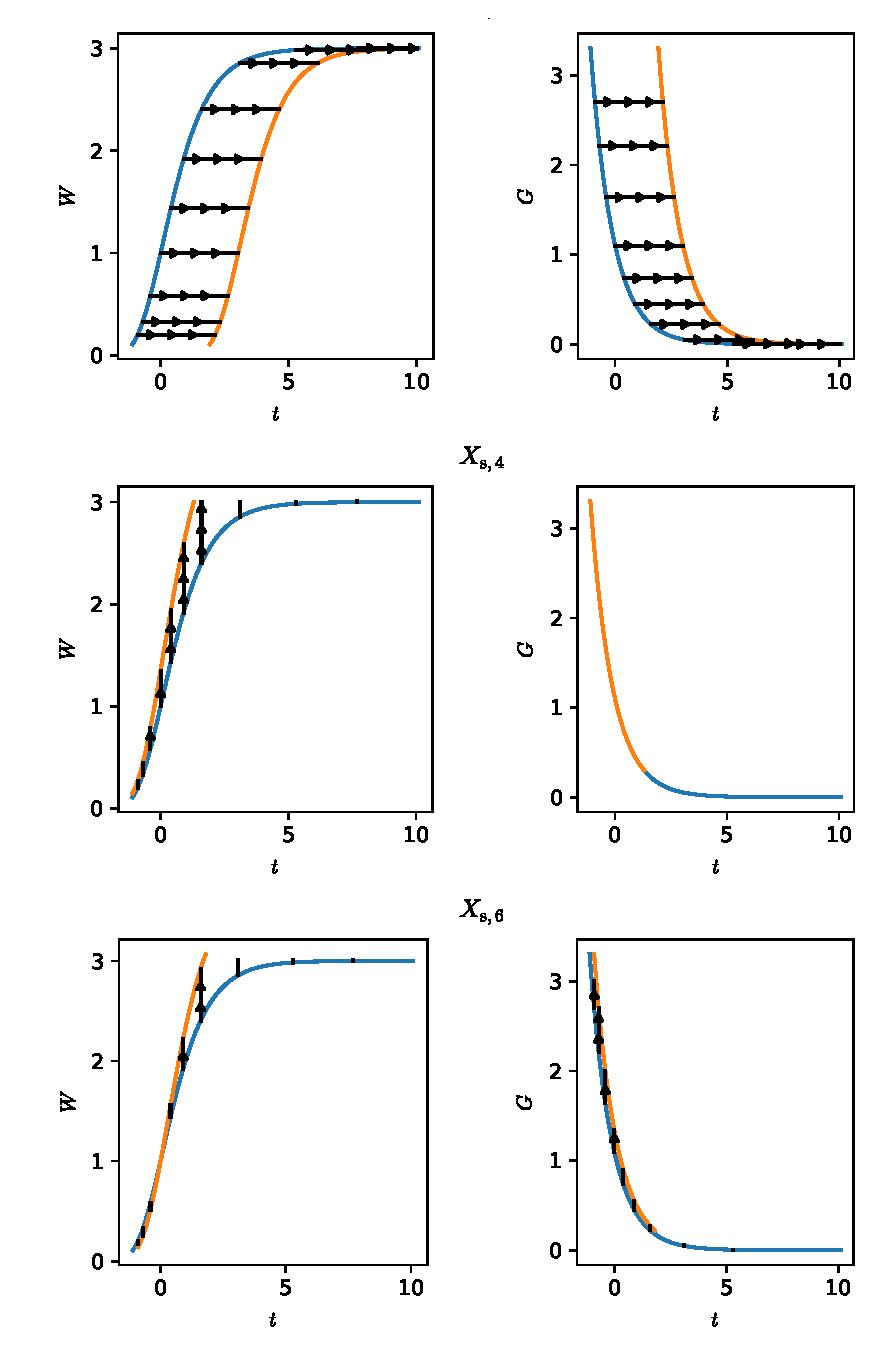
\includegraphics[width=.4772\textwidth]{images/gompertz-system-param}
  \caption{Representative transformations of the Lie groups corresponding to symmetry generators of the system Gompertz model found using the parameter independence method.}
  \label{fig:gompertz-system-param}
\end{figure}

\section{The Lotka--Volterra model}

The linearized symmetry condition \labelcref{eq:linearized-general-symmetry} is for the Lotka--Volterra model
\begin{subequations} \label[subequations]{eq:lotka-volterra-lin-symmetry-cond}
  \begin{align}
    \begin{split}
      \eta^1_t &+ \left(a N - b N\right) \left(\eta^1_{N} - \xi_t\right) + \left(c N P - d P\right) \eta^1_{P} - \left(a N - b N P\right)^2 \xi_{N} -\\
      &- \left(a N - b N P\right) \left(c N P - d P\right) \xi_{P} - \left(a - b P\right) \eta^1 + b N \eta^2 = 0
    \end{split}\\
    \begin{split}
      \eta^2_t &+ \left(a N - b N P\right) \eta^2_{N} + \left(c N P - d P\right) \left(\eta^2_{P} - \xi_t\right) -\\
      &- \left(a N - b N P\right) \left(c N P - d P\right) \xi_{N} - \left(c N P - d P\right)^2 \xi_{P} - c P \eta^1 -\\
      &- \left(c N - d\right) \eta^2 = 0.
    \end{split}
  \end{align}
\end{subequations}
The only symmetry found in \cref{ch:ansatze} independent in any parameter is \(\partial_t\).
Thus the parameter independence method should find that generator, and if any new symmetry generators are found they will be new.

\subsubsection{\texorpdfstring{\(a\)-independent symmetries}{a-independent symmetries}}

Decomposition of \cref{eq:lotka-volterra-lin-symmetry-cond} in \(a\) gives the parameter independence determining equations
\begin{subequations} \label[subequations]{eq:lotka-volterra-det-a}
  \begin{flalign}
    \diff{N}{t}, 1 & : & - N^{2} P^{2} b^{2} \xi_{N} - N P b \eta^1_{N} + N P b \xi_{t} + N b \eta^{2} + P b \eta^{1} +&&\\
    &&\quad+ \left(N P c - P d\right) \eta^1_{P} + \left(N^{2} P^{2} b c - N P^{2} b d\right) \xi_{P} + \eta^1_{t} &= 0 &\label{eq:lotka-volterra-det-a-a}\\
    \diff{N}{t}, a & : & 2 N^{2} P b \xi_{N} + N \eta^1_{N} - N \xi_{t} + \left(- N^{2} P c + N P d\right) \xi_{P} -&&\\
    &&\quad- \eta^{1} &= 0 &\label{eq:lotka-volterra-det-a-b}\\
    \diff{N}{t}, a^2 & : & - N^{2} \xi_{N} &= 0 &\label{eq:lotka-volterra-det-a-c}\\
    \diff{P}{t}, 1 & : & - N P b \eta^2_{N} - P c \eta^{1} + \left(- N c + d\right) \eta^{2} +&&\\
    &&\quad+  \left(- N P c + P d\right) \xi_{t} + \left(N P c - P d\right) \eta^2_{P} +&&\\
    &&\quad+ \left(N^{2} P^{2} b c - N P^{2} b d\right) \xi_{N} +&&\\
    &&\quad+ \left(- N^{2} P^{2} c^{2} + 2 N P^{2} c d - P^{2} d^{2}\right) \xi_{P} + \eta^2_{t} &= 0 &\label{eq:lotka-volterra-det-a-d}\\
    \diff{P}{t}, a & : & N \eta^2_{N} + \left(- N^{2} P c + N P d\right) \xi_{N} &= 0. &\label{eq:lotka-volterra-det-a-e}
  \end{flalign}
\end{subequations}
From \cref{eq:lotka-volterra-det-a-c,eq:lotka-volterra-det-a-e} it is clear that
\begin{subequations} \label[subequations]{eq:lotka-volterra-a-first-simplification}
  \begin{align}
    \eta^2 &= \eta^2(t, P)\\
    \xi &= \xi(t, P),
  \end{align}
\end{subequations}
and thus \cref{eq:lotka-volterra-det-a-d} can be written as
\begin{multline*}
  \eta^{1} = \left(- N + \frac{d}{c}\right) \xi_{t} + \left(N - \frac{d}{c}\right) \eta^2_{P} + \left(- \frac{N}{P} + \frac{d}{P c}\right) \eta^{2} +\\
  + \left(- N^{2} P c + 2 N P d - \frac{P d^{2}}{c}\right) \xi_{P} + \frac{\eta^2_{t}}{P c}.
\end{multline*}
Since neither \(\xi\) nor \(\eta^2\) depends on \(N\), and \(\eta^1\) thus only depends explicitly on \(N\), the remaining parameter independence determining equations \labelcref{eq:lotka-volterra-det-a-a,eq:lotka-volterra-det-a-b} can be decomposed further in \(N\) resulting in the equations
\begin{subequations}
  \begin{align}
    - 2 P c \xi_{P} &= 0 \label{eq:lotka-volterra-det-aN-a}\\
    P d \xi_{P} - \xi_{t} &= 0 \label{eq:lotka-volterra-det-aN-b}\\
    \frac{P d^{2} \xi_{P}}{c} + \frac{d \eta^2_{P}}{c} - \frac{d \xi_{t}}{c} - \frac{d \eta^{2}}{P c} - \frac{\eta^2_{t}}{P c} &= 0 \label{eq:lotka-volterra-det-aN-c}\\
    - P^{2} c^{2} \xi_{PP} - P c^{2} \xi_{P} &= 0 \label{eq:lotka-volterra-det-aN-d}\\
    3 P^{2} c d \xi_{PP} + P c \eta^2_{PP} - 2 P c \xi_{Pt} - c \eta^2_{P} + \left(2 P^{2} b c + 3 P c d\right) \xi_{P} + \frac{c \eta^{2}}{P} &= 0 \label{eq:lotka-volterra-det-aN-e}\\
    \begin{split}\label{eq:lotka-volterra-det-aN-f}
      - 3 P^{2} d^{2} \xi_{PP} + P b \xi_{t} - 2 P d \eta^2_{PP} + 4 P d \xi_{Pt} + 2 d \eta^2_{P} + \left(b - \frac{2 d}{P}\right) \eta^{2} +&\\
      + \left(- P^{2} b d - 3 P d^{2}\right) \xi_{P} - \xi_{tt} + 2 \eta^2_{Pt} - \frac{2 \eta^2_{t}}{P} &= 0
    \end{split}\\
    \begin{split}\label{eq:lotka-volterra-det-aN-g}
      \frac{P^{2} d^{3} \xi_{PP}}{c} + \frac{P b d \xi_{t}}{c} + \frac{P d^{2} \eta^2_{PP}}{c} - \frac{2 P d^{2} \xi_{Pt}}{c} + \left(\frac{b}{c} + \frac{2 d}{P c}\right) \eta^2_{t} +&\\
      + \left(\frac{b d}{c} + \frac{d^{2}}{P c}\right) \eta^{2} + \left(- \frac{P b d}{c} - \frac{d^{2}}{c}\right) \eta^2_{P} + \left(- \frac{P^{2} b d^{2}}{c} + \frac{P d^{3}}{c}\right) \xi_{P} +&\\
      + \frac{d \xi_{tt}}{c} - \frac{2 d \eta^2_{Pt}}{c} + \frac{\eta^2_{tt}}{P c} &= 0.
    \end{split}
  \end{align}
\end{subequations}
\Cref{eq:lotka-volterra-det-aN-a,eq:lotka-volterra-det-aN-b} gives that
\begin{equation*}
  \xi = c_1,
\end{equation*}
where \(c_1\) is an arbitrary constant.
Thus the remaining \cref{eq:lotka-volterra-det-aN-c,eq:lotka-volterra-det-aN-e,eq:lotka-volterra-det-aN-f,eq:lotka-volterra-det-aN-g} simplify to
\begin{subequations}
  \begin{align}
    \frac{d \eta^2_{P}}{c} - \frac{d \eta^{2}}{P c} - \frac{\eta^2_{t}}{P c} &= 0 \label{eq:lotka-volterra-det-aN-c-simp}\\
    P c \eta^2_{PP} - c \eta^2_{P} + \frac{c \eta^{2}}{P} &= 0 \label{eq:lotka-volterra-det-aN-e-simp}\\
    - 2 P d \eta^2_{PP} + 2 d \eta^2_{P} + \left(b - \frac{2 d}{P}\right) \eta^{2} + 2 \eta^2_{Pt} - \frac{2 \eta^2_{t}}{P} &= 0 \label{eq:lotka-volterra-det-aN-f-simp}\\
    \begin{split}
      \frac{P d^{2} \eta^2_{PP}}{c} + \left(\frac{b}{c} + \frac{2 d}{P c}\right) \eta^2_{t} + \left(\frac{b d}{c} + \frac{d^{2}}{P c}\right) \eta^{2} +&\\
      + \left(- \frac{P b d}{c} - \frac{d^{2}}{c}\right) \eta^2_{P} - \frac{2 d \eta^2_{Pt}}{c} + \frac{\eta^2_{tt}}{P c} &= 0.
    \end{split}
  \end{align}
\end{subequations}
\Cref{eq:lotka-volterra-det-aN-c-simp} has the general solution
\begin{equation*}
  \eta^{2} = F{\left(P e^{d t} \right)} e^{- d t}
\end{equation*}
for an arbitrary univariate function \(F\).
Thus \cref{eq:lotka-volterra-det-aN-e-simp,eq:lotka-volterra-det-aN-f-simp} can be further simplified to
\begin{subequations}
  \begin{align}
    P c e^{d t} F''{\left(P e^{d t} \right)} - c F'{\left(P e^{d t} \right)} + \frac{c F{\left(P e^{d t} \right)} e^{- d t}}{P} &= 0 \label{eq:lotka-volterra-det-aN-e-simp2}\\
    b F{\left(P e^{d t} \right)} e^{- d t} &= 0. \label{eq:lotka-volterra-det-aN-f-simp2}
  \end{align}
\end{subequations}
Thus it is clear from \cref{eq:lotka-volterra-det-aN-f-simp2} that
\begin{equation*}
  F \equiv 0
\end{equation*}
and hence the general solution to the parameter independence determining equations \labelcref{eq:lotka-volterra-det-a} is
\begin{align*}
  \xi &= c_1 \\
  \eta^1 &= 0\\
  \eta^2 &= 0
\end{align*}
which is spanned by the manifest generator
\begin{equation*}
  X_1 = \partial_t.
\end{equation*}

\subsubsection{\texorpdfstring{\(b\)-independent symmetries}{b-independent symmetries}}

Decomposition of \cref{eq:lotka-volterra-lin-symmetry-cond} in \(b\) gives the parameter independence determining equations
\begin{subequations} \label[subequations]{eq:lotka-volterra-det-b}
  \begin{flalign}
    \diff{N}{t}, 1 & : & - N^{2} a^{2} \xi_{N} + N a \eta^1_{N} - N a \xi_{t} - a \eta^{1} + \left(N P c - P d\right) \eta^1_{P} +&&\\&&+ \left(- N^{2} P a c + N P a d\right) \xi_{P} + \eta^1_{t} &= 0 &\label{eq:lotka-volterra-det-b-a}\\
    \diff{N}{t}, b & : & 2 N^{2} P a \xi_{N} - N P \eta^1_{N} + N P \xi_{t} + N \eta^{2} + P \eta^{1} +&&\\&&+ \left(N^{2} P^{2} c - N P^{2} d\right) \xi_{P} &= 0 &\label{eq:lotka-volterra-det-b-b}\\
    \diff{N}{t}, b^2 & : & - N^{2} P^{2} \xi_{N} &= 0 &\label{eq:lotka-volterra-det-b-c}\\
    \diff{P}{t}, 1 & : & N a \eta^2_{N} - P c \eta^{1} + \left(- N c + d\right) \eta^{2} + \left(- N P c + P d\right) \xi_{t} +&&\\&&+ \left(N P c - P d\right) \eta^2_{P} + \left(- N^{2} P a c + N P a d\right) \xi_{N} +&&\\&&+ \left(- N^{2} P^{2} c^{2} + 2 N P^{2} c d - P^{2} d^{2}\right) \xi_{P} + \eta^2_{t} &= 0 &\label{eq:lotka-volterra-det-b-d}\\
    \diff{P}{t}, b & : & - N P \eta^2_{N} + \left(N^{2} P^{2} c - N P^{2} d\right) \xi_{N} &= 0. &\label{eq:lotka-volterra-det-b-e}
  \end{flalign}
\end{subequations}
From \cref{eq:lotka-volterra-det-b-c,eq:lotka-volterra-det-b-e} it is clear that
\begin{subequations} \label[subequations]{eq:lotka-volterra-b-first-simplification}
  \begin{align}
    \xi &= \xi(t, P) \\
    \eta^2 &= \eta^2(t, P),
  \end{align}
\end{subequations}
and thus \cref{eq:lotka-volterra-det-b-d} can be written as
\begin{multline*}
  \eta^{1} = - N^{2} P c \xi_{P} + 2 N P d \xi_{P} + N \eta^2_{P} - N \xi_{t} -\\- \frac{N \eta^{2}}{P} - \frac{P d^{2} \xi_{P}}{c} - \frac{d \eta^2_{P}}{c} + \frac{d \xi_{t}}{c} + \frac{d \eta^{2}}{P c} + \frac{\eta^2_{t}}{P c}.
\end{multline*}
Since neither \(\xi\) nor \(\eta^2\) depends on \(N\), and \(\eta^1\) thus only depends explicitly on \(N\), the remaining parameter independence determining equations \labelcref{eq:lotka-volterra-det-b-a,eq:lotka-volterra-det-b-b} can be decomposed further in \(N\) resulting in the equations
\begin{subequations}
  \begin{flalign}
    1 & : & \frac{P^{2} d^{3} \xi_{PP}}{c} + \frac{P d^{2} \eta^2_{PP}}{c} - \frac{2 P d^{2} \xi_{Pt}}{c} - \frac{a d \xi_{t}}{c} +&&\\&&+ \left(- \frac{a}{P c} + \frac{2 d}{P c}\right) \eta^2_{t} + \left(\frac{a d}{c} - \frac{d^{2}}{c}\right) \eta^2_{P} +&&\\&&+ \left(- \frac{a d}{P c} + \frac{d^{2}}{P c}\right) \eta^{2} + \left(\frac{P a d^{2}}{c} + \frac{P d^{3}}{c}\right) \xi_{P} +&&\\&&+ \frac{d \xi_{tt}}{c} - \frac{2 d \eta^2_{Pt}}{c} + \frac{\eta^2_{tt}}{P c} &= 0 &\label{eq:lotka-volterra-det-bN-a}\\
    N & : & - 3 P^{2} d^{2} \xi_{PP} - 2 P d \eta^2_{PP} + 4 P d \xi_{Pt} - a \xi_{t} + 2 d \eta^2_{P} +&&\\&&+ \left(P a d - 3 P d^{2}\right) \xi_{P} - \xi_{tt} + 2 \eta^2_{Pt} - \frac{2 d \eta^{2}}{P} - \frac{2 \eta^2_{t}}{P} &= 0 &\label{eq:lotka-volterra-det-bN-b}\\
    N^{2} & : & 3 P^{2} c d \xi_{PP} + P c \eta^2_{PP} - 2 P c \xi_{Pt} - c \eta^2_{P} +&&\\&&+ \left(- 2 P a c + 3 P c d\right) \xi_{P} + \frac{c \eta^{2}}{P} &= 0 &\label{eq:lotka-volterra-det-bN-c}\\
    N^{3} & : & - P^{2} c^{2} \xi_{PP} - P c^{2} \xi_{P} &= 0 &\label{eq:lotka-volterra-det-bN-d}\\
    b & : & - \frac{P^{2} d^{2} \xi_{P}}{c} - \frac{P d \eta^2_{P}}{c} + \frac{P d \xi_{t}}{c} + \frac{d \eta^{2}}{c} + \frac{\eta^2_{t}}{c} &= 0 &\label{eq:lotka-volterra-det-bN-e}\\
    N b & : & - P^{2} d \xi_{P} + P \xi_{t} + \eta^{2} &= 0 &\label{eq:lotka-volterra-det-bN-f}\\
    N^{2} b & : & 2 P^{2} c \xi_{P} &= 0. &\label{eq:lotka-volterra-det-bN-g}
  \end{flalign}
\end{subequations}
Given \cref{eq:lotka-volterra-det-bN-g},
\begin{equation*}
  \xi_{P} = 0,
\end{equation*}
and thus \cref{eq:lotka-volterra-det-bN-f} gives that
\begin{equation*}
  \eta^{2} = - P \xi_t
\end{equation*}
Since the only functional dependence left is in \(t\) for the unknown function
\begin{equation*}
  \xi = \xi(t),
\end{equation*}
\cref{eq:lotka-volterra-det-bN-a,eq:lotka-volterra-det-bN-b,eq:lotka-volterra-det-bN-e} can be further decomposed in \(P\), resulting in the equations
\begin{flalign}
  1 & : & - \frac{a d \xi'}{c} + \left(\frac{a}{c} + \frac{d}{c}\right) \xi'' - \frac{\xi'''}{c} &= 0 &\label{eq:lotka-volterra-det-bNP-a}\\
  N & : & - a \xi' - \xi'' &= 0 &\label{eq:lotka-volterra-det-bNP-b}\\
  P b & : & \frac{d \xi'}{c} - \frac{\xi''}{c} &= 0. &\label{eq:lotka-volterra-det-bNP-c}
\end{flalign}
Unless \(a = -d\), which will not be the case as both parameters are strictly positive,
\begin{equation*}
  \xi' = 0,
\end{equation*}
and thus
\begin{equation*}
  \xi = c_1
\end{equation*}
for an arbitrary constant \(c_1\).
Thus, the general solution to the parameter independence determining equations \labelcref{eq:lotka-volterra-det-b} is
\begin{align*}
  \xi &= c_1 \\
  \eta^1 &= 0\\
  \eta^2 &= 0
\end{align*}
which is spanned by the manifest generator
\begin{equation*}
  X_1 = \partial_t.
\end{equation*}

\subsubsection{\texorpdfstring{\(c\) and \(d\)-independent symmetries}{c and d-independent symmetries}}

The only assumption about the parameters used in the calculations of \(a\) and \(b\)-independent symmetries are that the parameters are non-zero and that all parameters have the same sign (namely they are all positive).
Using the variable and parameter substitutions
\begin{align*}
  \tilde{N} &= P \\
  \tilde{P} &= N \\
  \tilde{a} &= -d \\
  \tilde{b} &= -c \\
  \tilde{c} &= -b \\
  \tilde{d} &= -a,
\end{align*}
the same calculations will thus hold for finding \(\tilde{a}\) and \(\tilde{b}\)-independent symmetries of the model after substitution, as all parameters still are non-zero and have the same sign.
Substituting back to the original model, the manifest symmetry generator
\begin{equation*}
  X_1 = \partial_t
\end{equation*}
must thus be the only \(c\) and \(d\)-independent symmetry generator.

\section{The Yildirim--Mackey lactose operon model}

As seen in the previous sections of this chapter, the naïve approach to solving the parameter independence determining equations requires guidance by a human; in general systems of first order PDE:s are not solvable in any algorithmic manner.
Additionally, as was seen in \cref{ch:ansatze} the linearized symmetry condition grows quickly with additional states.
As a consequence, it becomes unviable to solve the parameter independence determining equations for the Yildirim--Mackey lactose operon model the naïve way.
Not only will the decomposed equations be hard to get an overview on, leading to time consuming selection processes for the \enquote{next step} in the calculations.
The amount of calculations required will also grow as the amount of parameters of a model generally grows together with the number of states.

To exemplify this, the number of terms in the parameter independence determining equations for \(\alpha_M\)-independent generators is shown in \cref{tab:lac-operon-parameter-independence-terms}.
\begin{table}
  \centering
  \begin{tabular}{r@{ }rr@{ }l}
    \(\diff{M}{t}\),& \(1\):& 179& terms \\[1em]
    \(\diff{M}{t}\),& \(\alpha_M\):& 79& terms \\
    \(\diff{M}{t}\),& \(\left(\alpha_M\right)^2\):& 3& terms \\
    \(\diff{B}{t}\),& \(1\):& 112& terms \\
    \(\diff{B}{t}\),& \(\alpha_M\):& 6& terms \\
    \(\diff{L}{t}\),& \(1\):& 529& terms \\
    \(\diff{L}{t}\),& \(\alpha_M\):& 42& terms \\
    \(\diff{A}{t}\),& \(1\):& 307& terms \\
    \(\diff{A}{t}\),& \(\alpha_M\):& 18& terms \\
    \(\diff{P}{t}\),& \(1\):& 112& terms \\
    \(\diff{P}{t}\),& \(\alpha_M\):& 6& terms
  \end{tabular}
  \caption{Terms of the the parameter independence determining equations for \(\alpha_M\)-independent generators.}
  \label{tab:lac-operon-parameter-independence-terms}
\end{table}
In the process of refining forms of the unknown functions \(\xi, \eta^1, \dots, \eta^5\), each of these terms might in the worst case decompose into individual equations to be solved.
This extreme case would of course be easy to solve as all available undetermined functions and derivatives would have to be zero everywhere, but it nonetheless gives an upper bound on the number of the equations in the systems resulting from using the naïve approach.
For certain forms of equations, some first steps of simplification can be done algorithmically.
Looking at the earlier calculations for the Gompertz and Lotka--Volterra models, most have a common first step of eliminating dependence in one of the states for \(\xi\) and all but one of the \(\eta^i\) functions (see \cref{eq:system-gompertz-kG-first-simplification-1,eq:system-gompertz-kG-first-simplification-2,eq:lotka-volterra-a-first-simplification,eq:lotka-volterra-b-first-simplification}).
This pattern, which also fits for \(\alpha_M\)-independence, holds when only one equation (\cref{eq:lac-operon-a}) of the system of equations (\cref{eq:lac-operon}) is dependent on a parameter (\(\alpha_M\)) linearly.
If those conditions are true, \(\xi\) and all but one of the equations \(\eta^i\) will not be dependent on a state.
In the case of \(\alpha_M\)-independence, only \(\eta^1\) can be dependent on \(M\).
While this knowledge simplifies the parameter independence determining equations the determining system is still large, as seen in \cref{tab:lac-operon-parameter-independence-terms-simplified}, and not viable to solve the naïve way.
\begin{table}
  \centering
  \begin{tabular}{r@{ }rr@{ }l}
    \(\diff{M}{t}\),& \(1\):& 170& terms \\
    \(\diff{M}{t}\),& \(\alpha_M\):& 71& terms \\
    \(\diff{B}{t}\),& \(1\):& 100& terms \\
    \(\diff{L}{t}\),& \(1\):& 445& terms \\
    \(\diff{A}{t}\),& \(1\):& 271& terms \\
    \(\diff{P}{t}\),& \(1\):& 100& terms
  \end{tabular}
  \caption{Terms of the the parameter independence determining equations for \(\alpha_M\)-independent generators after an easy to find simplification.}
  \label{tab:lac-operon-parameter-independence-terms-simplified}
\end{table}


\chapter{Interpreting and using symmetries in biology} \label{ch:uses}

In the previous two chapters, two different methods were used to find symmetries of parametrized first order ODE:s.
However, finding symmetries has little to no value unless they can be used to better understand biological processes.
While some of the possible uses for symmetries have been mentioned in passing in earlier chapters, this chapter intends to explore these ideas more completely.
The chapter will consist of two parts.
In the first introductory part, an overview of how symmetries could fit into biological modeling is presented.
Most ideas will be open ended, as they constitute one or several research project on their own.
In the second part, one such use, namely the interpretation of symmetries as relating to invariants of the differential system, is explored for the biological models for which symmetries have been found.
It turns out, based on the mathematics in \cref{sec:lie-point-properties}, that the relation between invariants of the differential system and the symmetries thereof is quite straight forward for first order ODE systems.

\section{Symmetries as a tool in modeling} \label{sec:symmetries-as-tool}

\emph{
  Here there will be some discussion, similar to the one in the planning report and introduction, pertaining to the different use cases.
  Some notes that will be struck are: using symmetries for model construction, using symmetries to test models against data à la Fredrik and Johannes, using symmetries to compare models, how parameters are good to have in symmetries for data check vs. bad for general biological statements, conservation laws and their preservation in model reduction, using symmetries for full and partial integration of systems and looking at symmetries of subsystems of ODE:s.
}
% Using symmetry with param. ind. but Ovsiyannikov-like to get symmetries independent of arbitrary functions as parameters. Could then single cell variance be found in data looking at symmetries?

\section{Invariant solutions under symmetry of the Hill equation}

% TODO: This is a different kind of invariance, so a connection is needed
To better understand the underlying source of the Lie symmetry groups of the Hill equation, it is of interest to find curves invariant under the solution.
The reduced characteristic of the generator
\begin{equation}
  X_2 = - \left( (n-1) x + n y \right) \partial_\tau + y \partial_y
\end{equation}
is
\begin{align}
  \bar{Q} &= 
  \eta - \omega \xi = 
  y - \left( -\frac{y^n}{1+y^2} \right) \left( - \left( (n-1) \tau + n y \right) \right) =\\
  &= y \left(1 -\frac{y^{n-1} \left( (n-1) \tau + n y \right)}{1+y^2} \right).
\end{align}
Since solutions are invariant under a symmetry if the characteristic is 0 on the entire solution curve, invariant solutions must satisfy
\begin{equation}
  y \left(1 -\frac{y^{n-1} \left( (n-1) \tau + n y \right)}{1+y^n} \right) = 0.
\end{equation}
The solutions that meet this condition (aside from the trivial case \(y \equiv 0\)) must thus be on the form
\begin{equation}
  y^{n-1} \left( (n-1) \tau + n y \right) = 1+y^n,
\end{equation}
which is more clearly stated as
\begin{equation}
  (n-1) \left( \tau y^{n-1} + y^n \right) = 1.
\end{equation}
For all \(n>0\) except \(n=1\) such solutions exist, and take the form
\begin{equation} \label{eq:hill-invariants}
  \tau y^{n-1} + y^n = \frac{1}{n-1}.
\end{equation}
Additionally, since \(\tau\) is (dimensionless) time, any application of the model will have an initial condition on the form \(y(0) = y_0\).
By fixing \(\tau=0\) in \cref{eq:hill-invariants}, the initial condition of an invariant curve given any \(n>0, n\neq1\) is shown to be
\begin{equation}
  y(0) =\frac{1}{(n-1)^{1/n}}.
\end{equation}

\section{The structure of the full symmetry groups of the Gompertz models}

As discussed in \cref{sec:lie-point-properties}, all symmetries of first order systems of ODE:s can be separated in to two parts: the trivial component and the characteristic component.
Furthermore, the characteristic component's general form depends only on the invariants of the differential system.
Here this connection will be shown explicitly for all formulations of the Gompertz model, serving both as a case study and as a further investigation of the different formulations of the Gompertz model.

\subsection{The classical Gompertz model}

The symmetries of the classical Gompertz model found using an ansatz in \cref{ch:ansatze} were
\begin{align}
  X_{\text{c},1} &= e^{k_{G} t} \partial_t \\
  X_{\text{c},2} &= W e^{k_{G} t + e^{T_{i} k_{G}} e^{- k_{G} t}} \partial_t \\
  X_{\text{c},3} &= e^{- e^{T_{i} k_{G}} e^{- k_{G} t}} \partial_W \\
  X_{\text{c},f} &= \frac{f{\left(t \right)} e^{- T_{i} k_{G}} e^{k_{G} t}}{k_{G}} \partial_t + W f{\left(t \right)} \partial_W
\end{align}
and the symmetries found using parameter independence in \cref{ch:param-ind} were
\begin{align}
  X_{\text{c},1} &= e^{k_G t} \partial_t \\
  X_{\text{c},4} &= W \partial_W \\
  X_{\text{c},5} &= \partial_t - k_G W \ln(W) \partial_W.
\end{align}
The corresponding reduced characteristics of the symmetry generators are
\begin{align}
  \bar{Q}_{\text{c},1} &= -k_G e^{k_G T_i} W \\
  \bar{Q}_{\text{c},2} &= - k_G e^{k_{G} T_i + e^{-k_G (t - T_i)}} W^2 \\
  \bar{Q}_{\text{c},3} &= e^{- e^{- k_{G} \left(t - T_{i}\right)}} \\
  \bar{Q}_{\text{c},4} &= W \\
  \bar{Q}_{\text{c},5} &= - k_G W \ln(W) - k_G e^{-k_G (t - T_i)} W \\
  \bar{Q}_{\text{c},f} &= 0.
\end{align}
Thus it is clear that the symmetry generator \(X_{\text{c},f}\) is a trivial symmetry generator.
From the mathematical theory
\begin{equation}
  \bar{Q} = (\partial_W J)^{-1} I,
\end{equation}
where \(J\) is the universal invariant and \(I\) any invariant.
As the classical Gompertz model is a scalar first order ODE, the universal invariant is one-dimensional, and thus the quotient of two reduced characteristics must be an invariant.
Picking the reduced characteristics \(\bar{Q}_{\text{c},4}\) and \(\bar{Q}_{\text{c},5}\) that differ by more than a constant expression (assuming the parameters are constant),
\begin{equation}
  \frac{\bar{Q}_{\text{c},5}}{\bar{Q}_{\text{c},4}} = - k_G \left(\ln(W) + e^{-k_G (t - T_i)} \right) = I
\end{equation}
is an invariant since
\begin{equation}
  I_t + k_G e^{-k_G (t - T_i)} W I_W = k_G^2 e^{-k_G (t - T_i)} - k_G e^{-k_G (t - T_i)} W \frac{k_G}{W} = 0.
\end{equation}
For the particular case of scalar first order equations with known solutions such as the classical Gompertz ODE, the above described methodology is not the most direct path to finding such an invariant.
The formulation
\begin{equation}
  I_t + k_G e^{-k_G (t - T_i)} W I_W = 0
\end{equation}
of the invariance condition can be solved using the method of characteristics, which reformulates the problem as
\begin{equation}
  \frac{\dl{t}}{1} = \frac{\dl{W}}{k_G e^{-k_G (t - T_i)} W}
\end{equation}
which simplifies to
\begin{equation}
  \dl \left(e^{-k_G (t - T_i)} + \ln{W}\right) = 0
\end{equation}
leading to the equivalent invariant.
Returning to the task of determining the general structure of the group of all symmetries,
\begin{equation}
  J(t, W) = e^{-k_G (t - T_i)} + \ln{W}
\end{equation}
can be taken as the universal invariant.
Thus
\begin{equation}
  \partial_W J = \frac{1}{W}
\end{equation}
and
\begin{equation}
  \left(\partial_W J\right)^{-1} = W.
\end{equation}
Similarly, an arbitrary invariant \(I\) of the differential equation can be written as
\begin{equation}
  I(t, W) = F\left(e^{-k_G (t - T_i)} + \ln{W}\right)
\end{equation}
for and arbitrary function \(F\).
Thus, the reduced characteristic of any symmetry generator must have the form
\begin{equation} \label{eq:general-classical-gompertz-characteristic}
  \bar{Q} = W F\left(e^{-k_G (t - T_i)} + \ln{W}\right)
\end{equation}
and the general form for a symmetry generator is
\begin{equation} \label{eq:general-classical-gompertz-symmetry}
  X = \xi(t, W) \partial_t + W \left(k_G e^{-k_G (t - T_i)} \xi(t, W) + F\left(e^{-k_G (t - T_i)} + \ln{W}\right)\right) \partial_W
\end{equation}
for arbitrary functions \(\xi\) and \(F\).

\subsection{The autonomous Gompertz model}

The symmetries of the autonomous Gompertz model found using an ansatz in \cref{ch:ansatze} were
\begin{align}
  X_{\text{a},1} &= e^{k_G t} \ln(\frac{W}{A}) \partial_t \\
  X_{\text{a},2} &= e^{-k_G t} W \partial_W \\
  X_{\text{a},3} &= \ln(\frac{W}{A}) W \partial_W \\
  X_{\text{a},f} &= f(t) \partial_t - k_G f(t) \ln(\frac{W}{A}) W \partial_W
\end{align}
and the symmetries found using parameter independence in \cref{ch:param-ind} were
\begin{align}
  X_{\text{a},2} &= e^{-k_G t} W \partial_W \\
  X_{\text{a},3} &= \ln(\frac{W}{A}) W \partial_W \\
  X_{\text{a},4} &= \partial_t \\
  X_{\text{a},5} &= t \partial_t + \ln(\abs{\ln(\frac{W}{A})}) \ln(\frac{W}{A}) W \partial_W \\
  X_{\text{a},6} &= e^{-k_G t} \partial_t - k_G e^{-k_G t} \ln(W) W \partial_W.
\end{align}
The corresponding reduced characteristics of the symmetry generators are
\begin{align}
  \bar{Q}_{\text{c},1} &= k_G e^{k_G t} \left(\ln(\frac{W}{A})\right)^2 W \\
  \bar{Q}_{\text{c},2} &= e^{-k_G t} W \\
  \bar{Q}_{\text{c},3} &= \ln(\frac{W}{A}) W\\
  \bar{Q}_{\text{c},4} &= k_G \ln(\frac{W}{A}) W \\
  \bar{Q}_{\text{c},5} &= \ln(\abs{\ln(\frac{W}{A})}) \ln(\frac{W}{A}) W + k_G t \ln(\frac{W}{A}) W \\
  \bar{Q}_{\text{c},6} &= - k_G \ln(A) e^{-k_G t} W \\
  \bar{Q}_{\text{c},f} &= 0.
\end{align}
Just as for the classical Gompertz model, there are several ways to find a universal invariant of the autonomous Gompertz model.
Using the most straight-forward method,
\begin{equation}
  \frac{\bar{Q}_{\text{c},5}}{\bar{Q}_{\text{c},3}} = \ln(\abs{\ln(\frac{W}{A})}) + k_G t
\end{equation}
is an invariant, and thus
\begin{equation}
  J(t, W) = \ln(\abs{\ln(\frac{W}{A})}) + k_G t
\end{equation}
can be chosen as a universal invariant.
Thus
\begin{equation}
  \partial_W J = \frac{1}{\ln(\frac{W}{A}) W}
\end{equation}
and
\begin{equation}
  \left(\partial_W J\right)^{-1} = \ln(\frac{W}{A}) W.
\end{equation}
Using \cref{cor:reduced-characteristic-decomposition}, the reduced characteristic of symmetry generators of the autonomous Gompertz model thus has the general form
\begin{equation} \label{eq:general-autonomous-gompertz-characteristic}
  \bar{Q} = \ln(\frac{W}{A}) W F\left(\ln(\abs{\ln(\frac{W}{A})}) + k_G t\right),
\end{equation}
where \(F\) is an arbitrary function, with the general form for a symmetry generator being
\begin{equation} \label{eq:general-autonomous-gompertz-symmetry}
  X = \xi(t, W) \partial_t + \ln(\frac{W}{A}) W \left(-k_G \xi(t, W) + F\left(\ln(\abs{\ln(\frac{W}{A})}) + k_G t\right)\right) \partial_W
\end{equation}
for arbitrary functions \(\xi\) and \(F\).

\subsection{The system Gompertz model}

The symmetries of the system Gompertz model found using an ansatz in \cref{ch:ansatze} were
\begin{align}
  X_{\text{s},1} &= \partial_t \\
  X_{\text{s},2} &= - \frac{e^{k_{G} t}}{k_{G}} \partial_t + G e^{k_{G} t} \partial_G \\
  X_{\text{s},3} &= e^{k_{G} t} G \partial_t \\
  X_{\text{s},4} &= W \partial_W \\
  X_{\text{s},5} &= - \frac{W e^{- k_{G} t}}{k_{G}} \partial_W + e^{- k_{G} t} \partial_G
\end{align}
and the symmetries found using parameter independence in \cref{ch:param-ind} were
\begin{align}
  X_{\text{s},1} &= \partial_t \\
  X_{\text{s},4} &= W \partial_W \\
  X_{\text{s},6} &= \ln(W) W \partial_W + G \partial_G.
\end{align}
The corresponding reduced characteristics of the symmetry generators are
\begin{align}
  \bar{\vb{Q}}_{\text{s},1} &= \left(-W G, k_G G\right) \\
  \bar{\vb{Q}}_{\text{s},2} &= \left(\frac{e^{k_{G} t}}{k_{G}} W G, 0\right) \\
  \bar{\vb{Q}}_{\text{s},3} &= \left(- e^{k_{G} t} W G^2, k_G e^{k_{G} t} G^2\right) \\
  \bar{\vb{Q}}_{\text{s},4} &= \left(W, 0\right) \\
  \bar{\vb{Q}}_{\text{s},5} &= \left(- \frac{W e^{- k_{G} t}}{k_{G}}, e^{- k_{G} t} \right) \\
  \bar{\vb{Q}}_{\text{s},6} &= \left(\ln(W) W, G\right).
\end{align}
Since the system Gompertz model has two equations, two functionally independent invariants exist.
While it is a bit more cumbersome than in the scalar case to calculate invariants from the reduced characteristics, it is still possible.
However, in the particular case of the system Gompertz ODE, using the method of characteristics to solve the invariance condition is also a viable approach.
Both methods will be shown here to exemplify how the calculations are made for non-scalar ODE:s.

Using the reduced characteristics, one invariant can be found using the fact that
\begin{equation}
  \bar{\vb{Q}}_{\text{s},3} = e^{k_{G} t} G \left(-W G, k_G G\right) = e^{k_{G} t} G \bar{\vb{Q}}_{\text{s},1}
\end{equation}
implies that \(e^{k_{G} t} G\) is an invariant.
Using this invariant, all of the reduced characteristics \(\bar{\vb{Q}}_{\text{s},1}, \dots, \bar{\vb{Q}}_{\text{s},5}\) found using the ansatz method can be divided into two linearly independent\footnote{} sets of vectors % TODO: Write footnote
\begin{align}
  \bar{\vb{Q}}_{\text{s},1} &= \frac{\bar{\vb{Q}}_{\text{s},3}}{e^{k_{G} t} G} = \left(k_G e^{k_{G} t} G\right) \bar{\vb{Q}}_{\text{s},5} \\
  \frac{e^{k_{G} t} G}{k_G} \bar{\vb{Q}}_{\text{s},2} &= \bar{\vb{Q}}_{\text{s},4}.
\end{align}
\(-\bar{\vb{Q}}_{\text{s},1}\) and \(\bar{\vb{Q}}_{\text{s},4}\), being functionally independent, could be used to construct
\begin{equation}
  \begin{pmatrix}
    W & W G \\
    0 & -k_G G
  \end{pmatrix}
  = \left(\partial_{(W, G)} \vb{J}\right)^{-1},
\end{equation}
and thus a universal invariant would be the solutions to the differential equation
\begin{equation} \label{eq:universal-invariant-system-gompertz-hint}
  \partial_{(W, G)} \vb{J} =
  \begin{pmatrix}
    W & W G \\
    0 & -k_G G
  \end{pmatrix}^{-1}
\end{equation}
that also fulfill the original invariance condition
\begin{equation}
  \partial_{(t, W, G)} \vb{J} \cdot
  \begin{pmatrix}
    1 \\
    W G \\
    -k_G G
  \end{pmatrix}
  = 0.
\end{equation}
Thus, finding a universal invariant using only the reduced characteristics \(\bar{\vb{Q}}_{\text{s},1}, \dots, \bar{\vb{Q}}_{\text{s},5}\) found using the ansatz method is essentially the problem of finding invariants, but with \cref{eq:universal-invariant-system-gompertz-hint} serving as a hint.
But, using the reduced characteristic \(\bar{\vb{Q}}_{\text{s},6}\) found using the parameter independence method, this calculation can be avoided since
\begin{multline}
  \bar{\vb{Q}}_{\text{s},6} = \left(\ln(W) W, G\right) = \left(-\frac{W G}{k_G}, G\right) + \left(\ln(W) W + \frac{W G}{k_G}, 0\right) =\\= \frac{1}{k_G} \bar{\vb{Q}}_{\text{s},1} + \left(\ln(W) + \frac{G}{k_G}\right) \bar{\vb{Q}}_{\text{s},4}.
\end{multline}
\(\ln(W) + \frac{G}{k_G}\) must thus be an invariant, and since \(e^{k_{G} t} G\) and \(\ln(W) + \frac{G}{k_G}\) are functionally independent,
\begin{equation}
  \vb{J}(t, W, G) = \left(\ln(W) + \frac{G}{k_G}, \ln(e^{k_{G} t} G)\right) = \left(\ln(W) + \frac{G}{k_G}, k_G t + \ln(G)\right)
\end{equation}
must be a universal invariant.

Using the method of characteristics to solve the invariance condition
\begin{equation}
  I_t + W G I_W - k_G G I_G = 0,
\end{equation}
results in the reformulated problem
\begin{equation}
  \frac{\dl t}{1} = \frac{\dl W}{W G} = \frac{\dl G}{- k_G G}.
\end{equation}
The expression
\begin{equation}
  \frac{\dl W}{W G} = \frac{\dl G}{- k_G G}
\end{equation}
simplifies to
\begin{equation}
  \dl \left(\ln(W) + \frac{G}{k_G}\right) = 0,
\end{equation}
while
\begin{equation}
  \frac{\dl t}{1} = \frac{\dl G}{- k_G G}
\end{equation}
simplifies to
\begin{equation}
  \dl \left(k_G t + \ln(G)\right) = 0.
\end{equation}
Thus the universal invariant
\begin{equation} \label{eq:universal-invariant-system-gompertz}
  \vb{J}(t, W, G) = \left(\ln(W) + \frac{G}{k_G}, k_G t + \ln(G)\right)
\end{equation}
is once again found.

Using the universal invariant \labelcref{eq:universal-invariant-system-gompertz},
\begin{equation}
  \partial_{(W, G)} \vb{J} =
  \begin{pmatrix}
    \frac{1}{W} & \frac{1}{k_G} \\
    0 & \frac{1}{G}
  \end{pmatrix}
\end{equation}
and thus
\begin{equation}
  \left(\partial_{(W, G)} \vb{J}\right)^{-1} =
  \begin{pmatrix}
    W & - \frac{W G}{k_G} \\
    0 & G
  \end{pmatrix}.
\end{equation}
Using \cref{cor:reduced-characteristic-decomposition}, the reduced characteristic of any symmetry generator must thus have the form
\begin{equation} \label{eq:general-system-gompertz-characteristic}
  \bar{\vb{Q}} =
  \begin{pmatrix}
    W & - \frac{W G}{k_G} \\
    0 & G
  \end{pmatrix}
  \cdot
  \begin{pmatrix}
    F_1\left(\ln(W) + \frac{G}{k_G}, k_G t + \ln(G)\right) \\
    F_2\left(\ln(W) + \frac{G}{k_G}, k_G t + \ln(G)\right)
  \end{pmatrix},
\end{equation}
where \(F_1\) and \(F_2\) are arbitrary functions.
The general form of Lie point symmetry generators of the system Gompertz model is thus
\begin{align}
  X =& \xi(t, W, G) \partial_t + \\
  &+ \left(W G \xi(t, W, G) + W I_1(t, W, G) - \frac{W G}{k_G} I_2(t, W, G)\right) \partial_W + \\
  &+ \left(-k_G G \xi(t, W, G) + G I_2(t, W, G)\right) \partial_W,
\end{align}
where \(\xi\) is an arbitrary function and
\begin{align}
  I_1(t, W, G) &= F_1\left(\ln(W) + \frac{G}{k_G}, k_G t + \ln(G)\right) \\
  I_2(t, W, G) &= F_2\left(\ln(W) + \frac{G}{k_G}, k_G t + \ln(G)\right)
\end{align}
are invariants.

\subsection{Comparison of the Gompertz models}

With the general forms of the Gompertz model Lie point symmetries established, further insight to the relationship between the three models can be gained.
Since both the classical and the autonomous model exist in the same space (\(B \simeq \reals(t)\) and \(F \simeq \reals(W)\)), comparison between the scalar models is a natural starting point.

The trivial symmetry generator
\begin{equation}
  X_{\text{a},T} = \partial_t - k_G \ln(\frac{W}{A}) W \partial_W
\end{equation}
of the autonomous Gompertz model is symmetry of the classical Gompertz model, since
\begin{equation}
  -k_G \ln(\frac{W}{A}) W = W \left(k_G e^{-k_G (t - T_i)} - k_G \left(e^{-k_G (t - T_i)} + \ln(W)\right) + k_G \ln(A)\right),
\end{equation}
and thus \(X_{a,T}\) can be written on the general form \cref{eq:general-classical-gompertz-symmetry} of classical Gompertz symmetries, with \(F(x) = -k_G x + k_G \ln(A)\) and \(\xi(t, W) \equiv 1\).
Similarly, the trivial symmetry generator
\begin{equation}
  X_{\text{c},T} = \partial_t + k_G e^{-k_G (t - T_i)} W \partial_W
\end{equation}
of the classical Gompertz model can be written on the general form \cref{eq:general-autonomous-gompertz-symmetry} of autonomous Gompertz symmetries, since
\begin{equation}
  k_G e^{-k_G (t - T_i)} W = \ln(\frac{W}{A}) W \left(-k_G + k_G e^{k_G T_i} e^{-\left(\ln(\abs{\ln(\frac{W}{A})}) + k_G t\right)} + k_G\right). % TODO: Figure out abs problems
\end{equation}
The parameter \(k_G\) is assumed to have the same value in both models for these statements to hold, which is reasonable since the parametrization of all three models is done in such a way that \(k_G\) has the same effect on solution curves.
It is also worth noting that the parameters \(A\) and \(T_i\) are arbitrary values for the classical and autonomous Gompertz models respectively; they have no relation to the properties they represent when they are not part of the ODE formulation.
As long as \(A\) is considered an invariant of the classical Gompertz model and \(T_i\) is considered an invariant of the autonomous Gompertz model, the arbitrary invariant multipliers of the characteristic components of the respective symmetries can be chosen so that the vector field corresponding to the autonomous model is a symmetry of the classical model and vice versa.

The system Gompertz model can not as stringently be compared to the scalar models, but using some intuition the connection between the models and their symmetries can be shown to be quite straight forward.
Consider first the classical model and the system model.
In this case, \(G\) is \enquote{equal} to \(k_G e^{-k_G (t - T_i)}\).
The general form of the reduced characteristic for the classical model \labelcref{eq:general-classical-gompertz-characteristic} can then be seen as the first column and first invariant in the general form of the reduced characteristic for the system model \labelcref{eq:general-system-gompertz-characteristic}, since
\begin{equation}
  \bar{Q}_{\text{c}} = W F\left(e^{-k_G (t - T_i)} + \ln{W}\right)
\end{equation}
then has the same form as
\begin{equation}
  \bar{\vb{Q}}_{\text{s}} =
  \begin{pmatrix}
    W \\
    0
  \end{pmatrix}
  \cdot F_1\left(\ln(W) + \frac{G}{k_G}\right).
\end{equation}

Instead considering the autonomous and the system model, \(G\) is \enquote{equal} to \(-k_G \ln(\frac{W}{A}) W\)
The general form of the reduced characteristic for the autonomous model \labelcref{eq:general-autonomous-gompertz-characteristic} can then be seen as the second column and second invariant in the general form of the reduced characteristic for the system model \labelcref{eq:general-system-gompertz-characteristic}, since
\begin{equation}
  \bar{Q}_{\text{a}} = \ln(\frac{W}{A}) W F\left(\ln(\abs{\ln(\frac{W}{A})}) + k_G t\right)
\end{equation}
then has the same form as
\begin{equation}
  \bar{\vb{Q}}_{\text{s}} =
  \begin{pmatrix}
    - \frac{W G}{k_G} \\
    G
  \end{pmatrix}
  \cdot F_2\left(k_G t + \ln(G)\right).
\end{equation}

\section{The structure of the symmetry group of the Lotka--Volterra model}

The symmetries of the Lotka--Volterra model found using an ansatz in \cref{ch:ansatze} were
\begin{align}
  X_1 &= \partial_t \\
  X_2 &= \frac{-bNP + aN}{c} \partial_N + \frac{cNP - dP}{c} \partial_P \\
  X_3 &= \frac{t}{c} \partial_t + \frac{-btNP + atN}{c} \partial_N + \frac{ctNP - dtP}{c} \partial_P \\
  X_4 &= \frac{N}{c} \partial_t + \frac{-bcN^2P + acN^2 - bdNP + adN}{c^2} \partial_N + \frac{c^2N^2P - d^2P}{c^2} \partial_P \\
  X_5 &= \frac{P}{c} \partial_t + \frac{-bNP^2 + aNP}{c} \partial_N + \frac{cNP^2 - dP^2}{c} \partial_P
\end{align}
and the symmetries found using parameter independence in \cref{ch:param-ind} were
\begin{equation}
  X_1 = \partial_t.
\end{equation}
The corresponding reduced characteristics of the symmetry generators are
\begin{align}
  \bar{\vb{Q}}_1 &= - \left(a N - b N P, c N P - d P\right) \\
  \bar{\vb{Q}}_2 &= \frac{1}{c} \left(a N - b N P, c N P - d P\right) \\
  \bar{\vb{Q}}_3 &= 0 \\
  \bar{\vb{Q}}_4 &= \frac{d}{c^2}\left(aN- bNP, cNP - dP\right) \\
  \bar{\vb{Q}}_5 &= 0.
\end{align}
Thus only one of the potentially two forms of reduced characteristic (modulo multiplication by invariants) is found.
Furthermore, the reduced characteristics reveal no invariants by themselves.

Using the method of characteristics, one such invariant can be found with ease.
The invariance condition 
\begin{equation}
  I_t + \left(a N - b N P\right) I_N + \left(c N P - d P\right) I_P = 0
\end{equation}
results in the reformulated problem
\begin{equation} \label{eq:moc-lotka-volterra}
  \frac{\dl t}{1} = \frac{\dl N}{a N - b N P} = \frac{\dl P}{c N P - d P}.
\end{equation}
The second equality can be simplified to
\begin{equation}
  \frac{\dl N}{N} \left(c N - d\right) = \frac{\dl P}{P} \left(a - b P\right)
\end{equation}
which has the solution
\begin{equation} \label{eq:invariant-lotka-volterra}
  \dl \left(cN + bP - d \ln(N) - a \ln(P)\right) = 0.
\end{equation}
The first equality in \cref{eq:moc-lotka-volterra} does not have an explicit solution, for the same reason the Lotka--Volterra system itself does not have an explicit solution, but must instead be studied mostly using the invariant in \cref{eq:invariant-lotka-volterra} \cite{murray2002biology}.

Using the characteristics and invariants easily calculable, it can thus be concluded that all reduced characteristics
\begin{equation} \label{eq:lotka-volterra-characteristic}
  \bar{\vb{Q}} = F\left(cN + bP - d \ln(N) - a \ln(P)\right) \left(a N - b N P, c N P - d P\right)
\end{equation}
correspond to symmetry generators of the Lotka--Volterra predator prey model \labelcref{eq:lotka-volterra}, where \(F\) is an arbitrary function.
All generators on the form
\begin{align}
  X =& \xi(t, W, G) \partial_t + \\
  &+ \left(a N - b N P\right) \left(\xi(t, W, G) + F\left(cN + bP - d \ln(N) - a \ln(P)\right)\right) \partial_W + \\
  &+ \left(c N P - d P\right) \left(\xi(t, W, G) + F\left(cN + bP - d \ln(N) - a \ln(P)\right)\right) \partial_W
\end{align}
are thus symmetry generators of the Lotka--Volterra model.


\chapter{Discussion}

Looking at the non-trivial symmetries of the autonomous Gompertz model found by using ansätze
\begin{align}
  X_1 &= e^{k_G t} \ln(\frac{W}{A}) \partial_t \\
  X_2 &= e^{-k_G t} W \partial_W \\
  X_3 &= \ln(\frac{W}{A}) W \partial_W
\end{align}
compared to the non-trivial symmetries found using the parameter independence method
\begin{align}
  X_{\text{a},1} &= \partial_t \\
  X_{\text{a},2} &= t \partial_t + \ln(\ln(\frac{W}{A})) \ln(\frac{W}{A}) W \partial_W\\
  X_{\text{a},3} &= \ln(\frac{W}{A}) W \partial_W \\
  X_{\text{a},4} &= e^{-k_G t} \partial_t - k_G e^{-k_G t} \ln(W) W \partial_W\\
  X_{\text{a},6} &= e^{-k_G t} W \partial_W,
\end{align}
it is clear that the parameter independence method is useful.
% Using symmetry with param. ind. but Ovsiyannikov-like to get symmetries independent of arbitrary functions as parameters. Could then single cell variance be found in data looking at symmetries?


\appendix

\chapter{Computer algebra system} \label{app:computer-algebra}

% Fix description/listings interaction
% This breaks other parts of the document if defined in definitions.sty,
% so it is defined here instead.
% Based on: https://tex.stackexchange.com/a/93950
\makeatletter
  \let\orig@item\item

  \def\item{%
      \@ifnextchar{[}%
          {\lstinline@item}%
          {\orig@item}%
  }

  \begingroup
  \catcode`\]=\active
  \gdef\lstinline@item[{%
      \setbox0\hbox\bgroup
          \catcode`\]=\active
          \let]\lstinline@item@end
  }
  \endgroup

  \def\lstinline@item@end{%
      \egroup
      \orig@item[\usebox0]%
  }
\makeatother

% Raise asterisks in the code listings
% Based on: https://tex.stackexchange.com/a/303477
\makeatletter
\lst@CCPutMacro
    \lst@ProcessOther {"2A}{%
      \lst@ttfamily 
         {\raisebox{2pt}{*}}% used with ttfamily
         \textasteriskcentered}% used with other fonts
    \@empty\z@\@empty
\makeatother  

% Listings settings
\lstset{
   alsoletter={.},
   emph={
      sympy.Expr,
      ValueError,
      Generator,
      __call__,
      get_jet_space_basis,
      get_tangent_field,
      JetSpace,
      base_index,
      dependents,
      extension,
      original_total_space,
      decompose_generator,
      generator_on,
      get_lin_symmetry_cond,
      get_prolongations,
      lie_bracket,
      total_derivative,
      create_poly_ansatz,
      derivatives_sort_key,
      iter_wrapper,
      optional_iter,
      replace_consts,
      zip_strict,
   },
   emphstyle=\textbf,
   basicstyle=\linespread{0.83}\ttfamily,
}

\section*{\lstinline{symmetries}}

Calculate symmetries of ODE:s symbolically.

\subsection*{class \lstinline{symmetries.Generator(xis, etas, total_space)}}

   A local coordinate representation of an infinitesimal generator.

   \begin{description}
      \item[Parameters:] \leavevmode
        \begin{description}
            \item[\lstinline{xis (list[sympy.Expr])} -] The base space components of the tangent field.
            \item[\lstinline{etas (list[sympy.Expr])} -] The fiber components of the tangent field.
            \item[\lstinline{total_space (tuple[list[sympy.Expr], list["sympy.Expr"]])} -] The base\newline vectors of the total space on which the generator acts.
        \end{description}
   \end{description}

   \subsubsection*{\lstinline{__call__(expr, jet_space=None)}}

      Apply the generator on an expression on a jet space.

      \begin{description}
         \item[Parameters:] \leavevmode
           \begin{description}
               \item[\lstinline{expr (sympy.Expr)} -] The expression to apply the generator on.
               \item[\lstinline{jet_space (JetSpace, optional)} -] The jet space in which the expression lives.
           \end{description}
         \item[Returns:] The expression after application of the generator.
         \item[Return type:] \lstinline{sympy.Expr}
      \end{description}
   
   \subsubsection*{\lstinline{get_jet_space_basis(degree=0)}}

      Return the basis of a jet space on which the generator can act.

      The ordering is the same as the ordering of \lstinline{get_tangent_field()}.

      \begin{description}
         \item[Parameters:] \leavevmode
           \begin{description}
               \item[\lstinline{degree (int, optional)} -] The degree of the jet space.
           \end{description}
         \item[Returns:] The expressions corresponding to the basis vectors of the jet space.
         \item[Return type:] \lstinline{list[sympy.Expr]}
      \end{description}

   \subsubsection*{\lstinline{get_tangent_field(degree=0)}}

      Return the corresponding prolonged tangent field of the
      generator.

      The ordering is the same as the ordering of \lstinline{get_jet_space_basis()}.

      \begin{description}
         \item[Parameters:] \leavevmode
           \begin{description}
               \item[\lstinline{degree (int, optional)} -] The degree of the prolongation.
           \end{description}
         \item[Returns:] The expressions corresponding to the components of the (possibly prolonged) tangent field.
         \item[Return type:] \lstinline{list[sympy.Expr]}
      \end{description}

\subsection*{class \lstinline{symmetries.JetSpace(base_coord, fiber_coord, degree)}}

   A local coordinate representation of a jet space.

   \begin{description}
      \item[Parameters:] \leavevmode
        \begin{description}
            \item[\lstinline{base_coord (list[sympy.Expr])} -] The basis vectors of the base space.
            \item[\lstinline{fiber_coord (list[sympy.Expr])} -] The basis vectors of the fibers.
            \item[\lstinline{degree (int)} -] The degree of the created jet space. A degree of 0 corresponds to the total space.
        \end{description}     
   \end{description}

   \subsubsection*{\lstinline{base_index(base_symbol)}}

      Returns the derivative index for a coordinate in the base space.

      \begin{description}
         \item[Parameters:] \leavevmode
           \begin{description}
               \item[\lstinline{base_symbol (sympy.Expr)} -] The symbol to find the base index of.
           \end{description}
         \item[Returns:] The multiindex of the desired symbol in the base space.
         \item[Return type:] \lstinline{tuple[int, ...]} 
      \end{description}

   \subsubsection*{property \lstinline{dependents}}

      The fibers of the total space on which the jet space is built.

      \begin{description}
         \item[Returns:] The symbols of the original fibers.
         \item[Return type:] \lstinline{list[sympy.Expr]}
      \end{description}
   
   \subsubsection*{\lstinline{extension(new_degree)}}

      Creates a jet space on the same total space of a higher degree.

      \begin{description}
         \item[Parameters:] \leavevmode
           \begin{description}
               \item[\lstinline{new_degree (int)} -] The degree of the extended jet space. Must be higher than the current degree.
           \end{description}
         \item[Returns:] A deep copy of the jet space, with additional jet fibers of higher degree.
         \item[Return type:] \lstinline{JetSpace}
      \end{description}

   \subsubsection*{property \lstinline{original_total_space}}

      Return the coordinates of the total space on which the jet
      space is built

      \begin{description}
         \item[Returns:] The coordinates of the base space and fiber.
         \item[Return type:] \lstinline{tuple[list[sympy.Expr], list[sympy.Expr]]}
      \end{description}         

\subsection*{\lstinline{symmetries.decompose_generator(generator, basis)}}

   Decompose a generator by a basis of arbitrary constants or
   functions.

   Only decomposition of generators linear in the basis is
   implemented.

   \begin{description}
      \item[Parameters:] \leavevmode
        \begin{description}
            \item[\lstinline{generator (Generator)} -] The generator to decompose.
            \item[\lstinline{basis (list[sympy.Expr])} -] The arbitrary constants or functions in which the generator can be decomposed.
        \end{description}
      \item[Returns:] The generators that span the space the input generator was in.
      \item[Return type:] \lstinline{list[Generator]}
   \end{description}

\subsection*{\lstinline{symmetries.generator_on(total_space)}}

   Returns a initialization method for generators on the total space.

   Is meant to be used to reduce visual clutter in code where several
   generators on the same space are used.

   \begin{description}
      \item[Parameters:] \leavevmode
        \begin{description}
            \item[\lstinline{total_space (tuple[list[sympy.Expr], list[sympy.Expr]])} -] The base\newline vectors of the total space on which the generator acts.
        \end{description}
      \item[Returns:] A generator subclass without the total space argument in the initializer.
      \item[Return type:] \lstinline{Generator}
   \end{description}

\subsection*{\lstinline{symmetries.get_lin_symmetry_cond(diff_eqs, generator, jet_space,}\newline\lstinline{derivative_hints=None)}}

   Test if the linearized symmetry conditions hold differential
   equations.

   \begin{description}
      \item[Parameters:] \leavevmode
        \begin{description}
            \item[\lstinline{diff_eqs (sympy.Expr or list[sympy.Expr])} -] The differential equation(s)\newline expressed in jet space notation.
            \item[\lstinline{generator (Generator)} -] The generator corresponding to the Lie group of transformations to be tested.
            \item[\lstinline{jet_space (JetSpace)} -] The jet space on which the differential equations exist.
            \item[\lstinline{derivative_hints (sympy.Expr or list[sympy.Expr])} -] The highest order\newline derivative(s) that the differential equation(s) can be solved for.
        \end{description}

      \item[Returns:] The differential equation(s) that must hold for the infinitesimal generator to generate a Lie group of symmetries. The differential equations are expressed in jet space notation.
      \item[Return type:] \lstinline{sympy.Expr or list[sympy.Expr]}
   \end{description}

\subsection*{\lstinline{symmetries.get_prolongations(xis, etas, jet_space)}}

   Calculate the coefficients of a vector field prolonged over a jet
   space.

   The vector field is characterized by the coefficients of
   derivatives in the base space (xis) and the coefficients of
   derivatives in the fiber of the original fiber bundle (etas) from
   which the jet space is created.

   \begin{description}
      \item[Parameters:] \leavevmode
        \begin{description}
            \item[\lstinline{xis (list[sympy.Expr])} -] The base space components of the tangent field.
            \item[\lstinline{etas (list[sympy.Expr])} -] The fiber components of the tangent field.
            \item[\lstinline{jet_space (JetSpace)} -] The jet space on which the prolonged tangent field will be calculated.
        \end{description}
      \item[Returns:] The prolonged fiber expressions, ordered firstly by original fiber and secondly by corresponding derivative multiindex.
      \item[Return type:] \lstinline{dict[str, dict[tuple[int, ...], sympy.Expr]]}
   \end{description}

\subsection*{\lstinline{symmetries.lie_bracket(generator1, generator2)}}

   The Lie bracket of two generators in the same coordinate system.

   \begin{description}
      \item[Parameters:] \leavevmode
        \begin{description}
            \item[\lstinline{generator1 (Generator)} -] The left generator in the Lie bracket.
            \item[\lstinline{generator2 (Generator)} -] The right generator in the Lie bracket.
        \end{description}
      \item[Returns:] The Lie bracket of the two generators.
      \item[Return type:] \lstinline{Generator}
   \end{description}

\subsection*{\lstinline{symmetries.total_derivative(jet_exp, coordinate, domain)}}

   The total derivative of an expression in a coordinate.

   \begin{description}
      \item[Parameters:] \leavevmode
        \begin{description}
            \item[\lstinline{jet_exp (sympy.Expr)} -] The expression to be derived.
            \item[\lstinline{coordinate (sympy.Expr)} -] The coordinate to derive in. Should be one of the symbols of the base space.
            \item[\lstinline{domain (JetSpace)} -] The jet space in which \lstinline{jet_exp} exists.
        \end{description}
      \item[Returns:] The derived expression. This expression exists in the the (once) extended jet space compared to the domain of the derivative.
      \item[Return type:] \lstinline{sympy.Expr}
   \end{description}

\section*{\lstinline{symmetries.ansatz}}

Make ansätze for generators.

\subsection*{\lstinline{symmetries.ansatz.create_poly_ansatz(jet_space, degree=1)}}

   Create an infinitesimal generator that is polynomial in the
   components of a given jet space.

   \begin{description}
      \item[Parameters:] \leavevmode
        \begin{description}
            \item[\lstinline{jet_space (JetSpace)} -] The jet space on which the generator can act.
            \item[\lstinline{degree (int, optional)} -] The degree of the polynomials in all generator components.
        \end{description}
      \item[Returns:] The generator and arbitrary constants defined by the ansatz.
      \item[Return type:] \lstinline{tuple[Generator, list[sympy.Expr]]}
   \end{description}

\section*{\lstinline{symmetries.utils}}

Utilities for the main symmetries package.

\subsection*{\lstinline{symmetries.utils.derivatives_sort_key(function_order=None,}\newline\lstinline{argument_order=None)}}

   Ad hoc sort key for derivatives.

   \begin{description}
      \item[Parameters:] \leavevmode
        \begin{description}
            \item[\lstinline{function_order (list[sympy.Derivative], optional)} -] An ordering of the\newline functions.
            \item[\lstinline{argument_order (list[sympy.Expr], optional)} -] An ordering of the\newline arguments.
        \end{description}
      \item[Returns:] A sorting key for \lstinline{sympy.Derivative} that sorts firstly by function, secondly by derivative degree and thirdly by derivative arguments.
   \end{description}

\subsection*{\lstinline{symmetries.utils.iter_wrapper(possible_iter)}}

   Ensures that the argument can be treated as an iterable.

   \begin{description}
      \item[Parameters:] \leavevmode
        \begin{description}
            \item[\lstinline{possible_iter} -] A possible iterable.
        \end{description}
      \item[Returns:] A guaranteed iterable.
   \end{description}      

\subsection*{\lstinline{symmetries.utils.optional_iter(func)}}

   Decorator that allows the first argument and return value to be
   optionally treated as iterables.

   \begin{description}
      \item[Parameters:] \leavevmode
        \begin{description}
            \item[\lstinline{func} -] The function should take an iterable as first argument and return an iterable.
        \end{description}
      \item[Returns:] The decorated function will accept either a single element or an iterable as first argument, and will return a single element or an iterable depending on the input type.
   \end{description}

\subsection*{\lstinline{symmetries.utils.replace_consts(exprs, new_const_name)}}

   Replace arbitrary constant from eg. \lstinline{sympy.dsolve}.

   \begin{description}
      \item[Parameters:] \leavevmode
        \begin{description}
            \item[\lstinline{exprs (sympy.Expr or list[sympy.Expr])} -] The expression(s) to\newline replace constants in.
            \item[\lstinline{new_const_name (str)} -] The new base name to give to the constants. E.g.\newline \lstinline{new_const_name = r"\\alpha"} will result in constants \lstinline|r"\alpha_{1}"|,\newline \lstinline|r"\alpha_{2}"| etc.
        \end{description}
      \item[Returns:] The new expressions and all the new constants.
      \item[Return type:] \lstinline{tuple[sympy.Expr or list[sympy.Expr], list[sympy.Expr]]}
   \end{description}

\subsection*{\lstinline{symmetries.utils.zip_strict(*iters)}}

   Zip two iterables and ensure that they are equal. Will be replaced
   with \lstinline{strict=True} argument in Python 3.10.

   \begin{description}
      \item[Parameters:] \leavevmode
        \begin{description}
          \item[\lstinline{*iters} -] Any number of iterables.
        \end{description}
      \item[Returns:] An iterable through tuples of the ingoing iterables.
      \item[Raises:] \leavevmode
      \begin{description}
        \item[\lstinline{ValueError} -] if the iterables have different lengths.
      \end{description}
   \end{description}     


\printbibliography[heading=bibintoc]

\end{document}
